% =====================================================================================
%  AI-Powered Smart Home Automation Using IoT, Machine Learning and
%  Retrieval-Augmented Generation  --  Project Report
%
%  Self-contained, single-file report. Compile with pdfLaTeX (Overleaf default).
%  Run pdfLaTeX twice so the table of contents, lists and cross-references resolve.
%
%  EDIT THE PLACEHOLDERS IN THE "PROJECT DETAILS" BLOCK BELOW BEFORE SUBMISSION.
% =====================================================================================
\documentclass[12pt,a4paper,oneside]{report}

% ------------------------------------------------------------------ packages
\usepackage[T1]{fontenc}
\usepackage[utf8]{inputenc}
\usepackage{lmodern}
\usepackage{microtype}
\usepackage[a4paper,left=3cm,right=2.5cm,top=2.5cm,bottom=2.5cm]{geometry}
\usepackage{setspace}
\usepackage{amsmath,amssymb}
\usepackage{graphicx}
\usepackage{xcolor}
\usepackage{tikz}
\usetikzlibrary{arrows.meta,positioning,shapes.geometric,fit,calc,backgrounds}
\usepackage{booktabs,longtable,tabularx,array,multirow}
\usepackage{listings}
\usepackage{float}
\usepackage{caption}
\usepackage{enumitem}
\usepackage{fancyhdr}
\usepackage{algorithm}
\usepackage{algpseudocode}
\usepackage{url}
\usepackage[hidelinks,bookmarksnumbered]{hyperref}

% ------------------------------------------------------------------ PROJECT DETAILS (edit these)
\newcommand{\ProjectTitle}{AI-Powered Smart Home Automation Using IoT, Machine Learning and Retrieval-Augmented Generation}
\newcommand{\StudentOne}{[Student Name 1]}
\newcommand{\RollOne}{[Roll No. 1]}
\newcommand{\StudentTwo}{[Student Name 2]}
\newcommand{\RollTwo}{[Roll No. 2]}
\newcommand{\StudentThree}{[Student Name 3]}
\newcommand{\RollThree}{[Roll No. 3]}
\newcommand{\GuideName}{[Project Guide Name and Designation]}
\newcommand{\HODName}{[Head of Department Name]}
\newcommand{\PrincipalName}{[Principal Name]}
\newcommand{\Department}{[Department of Computer Engineering / Information Technology]}
\newcommand{\College}{[Name of the College / Institute]}
\newcommand{\University}{[Name of the University]}
\newcommand{\Degree}{[Bachelor of Engineering / Bachelor of Technology]}
\newcommand{\AcademicYear}{[20XX--20XX]}
\newcommand{\Place}{[Place]}
\newcommand{\SubmissionDate}{[Date of submission]}

% ------------------------------------------------------------------ helper macros
% \code{...} prints identifiers (underscores, slashes) verbatim in typewriter type. Do not put % or # inside.
\newcommand{\code}[1]{\texttt{\detokenize{#1}}}
% \api{...} prints a URL path and may break after slashes. Do not put % or # inside.
\newcommand{\api}[1]{\path{#1}}
\urlstyle{tt}
\newcommand{\degC}{$^{\circ}$C}
\newcommand{\simulated}{\textit{(simulated data)}}

% ------------------------------------------------------------------ look and feel
\setstretch{1.2}
\setlength{\parindent}{0pt}
\setlength{\parskip}{0.55em}
\renewcommand{\arraystretch}{1.18}
\setlist{itemsep=0.2em,topsep=0.3em}
\emergencystretch=3em
\captionsetup{font=small,labelfont=bf}

\setlength{\headheight}{14.5pt}
\pagestyle{fancy}
\fancyhf{}
\fancyhead[L]{\small\nouppercase{\leftmark}}
\fancyfoot[C]{\thepage}
\renewcommand{\headrulewidth}{0.3pt}
\fancypagestyle{plain}{\fancyhf{}\fancyfoot[C]{\thepage}\renewcommand{\headrulewidth}{0pt}}

\lstset{
  basicstyle=\ttfamily\footnotesize,
  breaklines=true,
  breakatwhitespace=false,
  frame=single,
  rulecolor=\color{black!35},
  backgroundcolor=\color{black!3},
  columns=fullflexible,
  keepspaces=true,
  showstringspaces=false,
  xleftmargin=0.5em,
  xrightmargin=0.5em
}

% ------------------------------------------------------------------ TikZ styles
\tikzset{
  >={Stealth[length=2.2mm]},
  box/.style={draw=black!70, rounded corners=2pt, align=center, font=\footnotesize, inner sep=4pt, minimum height=7mm, fill=blue!6},
  dev/.style={box, fill=orange!14},
  broker/.style={box, fill=green!12},
  svc/.style={box, fill=blue!8},
  store/.style={box, fill=yellow!16},
  ext/.style={box, fill=gray!14, dashed},
  ui/.style={box, fill=purple!9},
  dec/.style={draw=black!70, diamond, aspect=2.2, align=center, font=\scriptsize, inner sep=1pt, fill=red!7},
  state/.style={draw=black!70, circle, align=center, font=\scriptsize, inner sep=2pt, minimum size=13mm, fill=blue!6},
  lbl/.style={font=\scriptsize, midway, fill=white, inner sep=1pt},
  group/.style={draw=black!45, dashed, rounded corners=4pt, inner sep=6pt},
  entity/.style={draw=black!70, rectangle, align=left, font=\scriptsize, inner sep=3pt, fill=blue!5},
  flow/.style={->, thick}
}

\begin{document}

% =====================================================================================
%  FRONT MATTER
% =====================================================================================
\pagenumbering{roman}

% ------------------------------------------------------------------ title page
\begin{titlepage}
\centering
\setstretch{1.15}
{\large\bfseries A PROJECT REPORT\par}
\vspace{0.3cm}
{\normalsize on\par}
\vspace{0.6cm}
{\LARGE\bfseries \ProjectTitle\par}
\vspace{0.9cm}
{\normalsize Submitted in partial fulfilment of the requirements for the award of the degree of\par}
\vspace{0.3cm}
{\large\bfseries \Degree\par}
\vspace{0.2cm}
{\normalsize in\par}
{\large\bfseries \Department\par}
\vspace{0.9cm}
{\normalsize Submitted by\par}
\vspace{0.3cm}
\begin{tabular}{lc}
\textbf{\StudentOne} & \RollOne\\
\textbf{\StudentTwo} & \RollTwo\\
\textbf{\StudentThree} & \RollThree
\end{tabular}
\vspace{0.9cm}

{\normalsize Under the guidance of\par}
{\large\bfseries \GuideName\par}
\vspace{1.2cm}
{\large\bfseries \College\par}
{\normalsize \University\par}
\vspace{0.4cm}
{\normalsize Academic Year \AcademicYear\par}
\end{titlepage}

% ------------------------------------------------------------------ certificate
\chapter*{Certificate}
\addcontentsline{toc}{chapter}{Certificate}
\setstretch{1.35}
This is to certify that the project report entitled
\textbf{``\ProjectTitle''} is a bona fide record of the work carried out by
\textbf{\StudentOne} (\RollOne), \textbf{\StudentTwo} (\RollTwo) and \textbf{\StudentThree} (\RollThree)
in partial fulfilment of the requirements for the award of the degree of \textbf{\Degree} in
\textbf{\Department} of \textbf{\College}, \University, during the academic year \AcademicYear.

The work embodied in this report has not been submitted to any other university or institute for the award of any degree or diploma.

\vspace{2.2cm}
\begin{tabularx}{\textwidth}{XXX}
\textbf{Project Guide} & \textbf{Head of Department} & \textbf{Principal}\\[0.2cm]
\GuideName & \HODName & \PrincipalName\\[1.4cm]
Signature: \rule{3cm}{0.4pt} & Signature: \rule{3cm}{0.4pt} & Signature: \rule{3cm}{0.4pt}
\end{tabularx}

\vspace{1.4cm}
\textbf{External Examiner:} \rule{5cm}{0.4pt}\hfill \textbf{Date:} \SubmissionDate

% ------------------------------------------------------------------ declaration
\chapter*{Declaration}
\addcontentsline{toc}{chapter}{Declaration}
We hereby declare that the project report entitled \textbf{``\ProjectTitle''}, submitted to \College, \University, in partial fulfilment of the requirements for the award of the degree of \Degree\ in \Department, is a record of original work carried out by us under the guidance of \GuideName.

We further declare that, to the best of our knowledge, this report does not contain material previously published or written by another person, except where due reference is made in the text, and that it has not been submitted, in whole or in part, for any other degree or diploma.

\vspace{1.5cm}
\begin{tabularx}{\textwidth}{Xl}
\textbf{Place:} \Place & \StudentOne\ (\RollOne)\\[0.4cm]
\textbf{Date:} \SubmissionDate & \StudentTwo\ (\RollTwo)\\[0.4cm]
 & \StudentThree\ (\RollThree)
\end{tabularx}

% ------------------------------------------------------------------ acknowledgement
\chapter*{Acknowledgement}
\addcontentsline{toc}{chapter}{Acknowledgement}
We would like to express our sincere gratitude to our project guide, \GuideName, for the guidance, encouragement and constructive criticism that shaped this work from the initial idea to the final report.

We thank \HODName, Head of the \Department, and \PrincipalName, Principal of \College, for providing the facilities and the academic environment that made this project possible. We are also grateful to the faculty and staff of the department for their support.

Finally, we thank our families and friends for their patience and encouragement throughout the project.

\vspace{1.2cm}
\hfill \StudentOne, \StudentTwo, \StudentThree

% ------------------------------------------------------------------ abstract
\chapter*{Abstract}
\addcontentsline{toc}{chapter}{Abstract}
\setstretch{1.2}
Home automation systems are usually either simple remote controls without any understanding of the data they collect, or cloud products that hide how decisions are made. This project builds a self-hosted, explainable smart-home platform that combines an ESP32-S3 sensor node, an MQTT message broker, a Spring Boot backend with a PostgreSQL database, a React web application, classical machine-learning components written in Java, and a retrieval-augmented generation (RAG) assistant backed by PostgreSQL with the pgvector extension.

The ESP32-S3 node reads a DHT22 temperature and humidity sensor, a PIR motion sensor and an MQ-2 gas sensor, drives two indicator LEDs, and keeps a locally implemented gas warning that works without any network. Devices are claimed with one-time pairing codes and then authenticate to the broker with their own credentials. The backend validates and stores telemetry, derives device presence, and sends authenticated, expiring, acknowledged commands for the two LEDs; the gas warning LED can never be switched off remotely. A rule-based automation engine supports sensor and schedule rules with priorities, cooldowns and an audit trail. A logistic-regression model trained with iteratively reweighted least squares predicts occupancy (PIR activity) from time of day and day of week and is evaluated on a chronological hold-out set against a baseline; robust statistics (median and median absolute deviation) detect unusual, missing, stuck, impossible and stale sensor readings with a stored explanation. A chat assistant retrieves the user's own records by vector similarity, builds a fenced prompt, checks the answer against its sources, and may propose automation rules that take effect only after explicit approval. Further modules provide Away and Night security modes with an event history, a device digital twin that compares confirmed and reported state, evidence-based recommendations that also require approval, and an authenticated system-status view.

The backend is verified by 372 automated tests, all passing, and the integration with real PostgreSQL and Mosquitto instances was exercised with scripts that stand in for devices.
\textbf{Scope of validation (disclosure):} the ESP32-S3 firmware compiles and its logic is unit-tested on a PC, but it has \emph{not} been run on a physical ESP32 board, and the assistant has \emph{not} been validated with a real large language model (a scripted fake and a local stub server were used instead). All machine-learning accuracy figures in this report come from simulated data and are not claims about real homes.

\medskip
\textbf{Keywords:} Internet of Things, ESP32-S3, MQTT, Spring Boot, PostgreSQL, pgvector, machine learning, anomaly detection, retrieval-augmented generation, smart home, digital twin.

\setstretch{1.2}
\tableofcontents
\clearpage
\listoffigures
\clearpage
\listoftables
\clearpage

% ------------------------------------------------------------------ abbreviations
\chapter*{List of Abbreviations}
\addcontentsline{toc}{chapter}{List of Abbreviations}
\begin{tabularx}{\textwidth}{lX}
\toprule
\textbf{Abbreviation} & \textbf{Meaning}\\
\midrule
ACL & Access Control List\\
ADC & Analog-to-Digital Converter\\
API & Application Programming Interface\\
AUC & Area Under the ROC Curve\\
DHT22 & Digital humidity and temperature sensor\\
ER & Entity--Relationship\\
IoT & Internet of Things\\
IRLS & Iteratively Reweighted Least Squares\\
JPA & Jakarta Persistence API\\
JSON & JavaScript Object Notation\\
JWT & JSON Web Token\\
LLM & Large Language Model\\
MAD & Median Absolute Deviation\\
ML & Machine Learning\\
MQ-2 & Combustible gas and smoke sensor module\\
MQTT & Message Queuing Telemetry Transport\\
NVS & Non-Volatile Storage (ESP32 flash key--value store)\\
PIR & Passive Infrared (motion sensor)\\
QoS & Quality of Service (MQTT)\\
RAG & Retrieval-Augmented Generation\\
REST & Representational State Transfer\\
SHA-256 & Secure Hash Algorithm, 256-bit\\
TTL & Time To Live\\
UUID & Universally Unique Identifier\\
\bottomrule
\end{tabularx}

\clearpage
\pagenumbering{arabic}
\setcounter{page}{1}

% =====================================================================================
%  CHAPTER 1
% =====================================================================================
\chapter{Introduction}

\section{Background}
The Internet of Things (IoT) connects small, inexpensive sensing and actuating devices to networks so that physical conditions such as temperature, humidity, motion or air quality can be observed and acted upon remotely. In the home, this has produced a large class of ``smart home'' products: sensors that report to a phone application, lamps and plugs that can be switched from anywhere, and rules such as ``turn this on at sunset''.

Most such systems stop at remote control and fixed schedules. They collect a stream of measurements but do very little with it: they do not learn when a room is normally occupied, they do not notice that a sensor has frozen or that a device has silently dropped off the network, and they cannot answer a plain-language question such as ``what was the temperature in the living room this morning, and was anything unusual?''. Where such features exist, they commonly run in a vendor's cloud, which makes it hard for the owner to see what the system knows, how it reached a conclusion, or who else can read the data.

This project explores a different design: a self-hosted platform in which every layer is open, every decision can be explained from stored data, and the more ``intelligent'' features (prediction, anomaly detection, a chat assistant, recommendations) are advisory and cannot override safety-critical behaviour that lives on the device itself.

\section{Motivation}
Three observations motivate the work.
\begin{enumerate}
  \item \textbf{Data without understanding.} A sensor node that reports every thirty seconds produces thousands of rows per day. Without statistical analysis these rows are just storage.
  \item \textbf{Safety must not depend on software layers.} A gas sensor is useful only if its warning works when Wi-Fi, the server or any AI component is unavailable. The architecture therefore keeps the gas warning entirely on the microcontroller and treats everything else as advisory.
  \item \textbf{AI answers must be grounded and controllable.} A language model that is allowed to guess readings or to change settings on its own is a liability in a home. The assistant here only answers from retrieved records, shows its sources, flags numbers it cannot find in those sources, and can only \emph{propose} changes that a human must approve.
\end{enumerate}

\section{Overview of the Proposed System}
The system has five cooperating parts (Figure~\ref{fig:overview-simple} gives the picture; Chapter~\ref{ch:architecture} describes it in detail):
\begin{itemize}
  \item an \textbf{ESP32-S3 sensor node} with a DHT22, a PIR sensor, an MQ-2 gas sensor and two LEDs;
  \item an \textbf{Eclipse Mosquitto MQTT broker} with per-device accounts and access control;
  \item a \textbf{Spring Boot backend} (Java 21) that owns users, devices, telemetry, commands, automation, machine learning, the assistant, security modes and system status, in one deployable application (a modular monolith);
  \item a \textbf{PostgreSQL database} with the pgvector extension, whose schema is managed by Flyway migrations;
  \item a \textbf{React web application} (TypeScript, Vite, Tailwind CSS) for registration, device management, automation, ML insights, the assistant and the dashboard.
\end{itemize}

\begin{figure}[H]
\centering
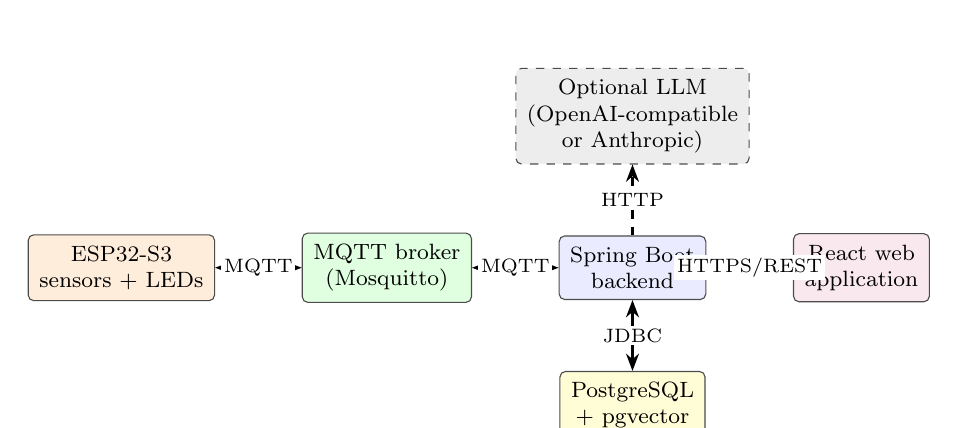
\begin{tikzpicture}[node distance=9mm and 11mm]
  \node[dev] (esp) {ESP32-S3\\sensors + LEDs};
  \node[broker, right=of esp] (mq) {MQTT broker\\(Mosquitto)};
  \node[svc, right=of mq] (be) {Spring Boot\\backend};
  \node[store, below=of be] (db) {PostgreSQL\\+ pgvector};
  \node[ui, right=of be] (web) {React web\\application};
  \node[ext, above=of be] (llm) {Optional LLM\\(OpenAI-compatible\\or Anthropic)};
  \draw[<->, thick] (esp) -- node[lbl]{MQTT} (mq);
  \draw[<->, thick] (mq) -- node[lbl]{MQTT} (be);
  \draw[<->, thick] (be) -- node[lbl]{JDBC} (db);
  \draw[<->, thick] (be) -- node[lbl]{HTTPS/REST} (web);
  \draw[->, thick, dashed] (be) -- node[lbl]{HTTP} (llm);
\end{tikzpicture}
\caption{The system at a glance. The language model is optional and external; everything else runs on the owner's machine.}
\label{fig:overview-simple}
\end{figure}

\section{Scope of the Work}
The work covers the full path from a physical sensor to a user decision: firmware, messaging, persistence, security, automation, machine learning, retrieval-augmented question answering and a web interface. It was developed incrementally in nine stages (called \emph{chunks} throughout this report), each of which was tested before the next began (Section~\ref{sec:chunks}).

The following are explicitly \emph{outside} the scope: cloud deployment, mobile applications, TLS on the MQTT link, OTA firmware updates, energy metering, and any form of certified alarm or gas-safety function.

\section{Organisation of the Report}
Chapter~\ref{ch:problem} states the problem and the objectives. Chapter~\ref{ch:requirements} lists the requirements. Chapter~\ref{ch:architecture} presents the architecture and data flows. Chapters~\ref{ch:hardware} and~\ref{ch:tech} describe the hardware and the technology stack. Chapter~\ref{ch:features} explains each implemented feature (Chunks~1--9). Chapters~\ref{ch:database}, \ref{ch:api} and~\ref{ch:algorithms} cover the database, the API and the algorithms. Chapter~\ref{ch:security} analyses security. Chapters~\ref{ch:install} and~\ref{ch:testing} explain installation and give the verified test results. Chapters~\ref{ch:limits}--\ref{ch:conclusion} discuss limitations, future scope and conclusions.

% =====================================================================================
%  CHAPTER 2
% =====================================================================================
\chapter{Problem Statement and Objectives}
\label{ch:problem}

\section{Problem Statement}
Existing low-cost home-automation setups suffer from the following weaknesses.
\begin{enumerate}
  \item They report raw values but do not analyse them, so unusual, missing, frozen or impossible readings and silent devices go unnoticed.
  \item Remote control is often added without strong ownership checks, command expiry or acknowledgement, so a command may be replayed, sent to the wrong device or silently lost.
  \item Gas or smoke warnings are sometimes routed through the network or the cloud, so the warning fails when the network fails.
  \item Intelligent features are opaque: the owner cannot see the data, the algorithm or the evidence behind a prediction or a suggestion.
  \item Chat assistants built on large language models tend to invent facts, can be manipulated by text stored in their context (prompt injection), and may be given the power to act without confirmation.
\end{enumerate}

The problem addressed here is therefore: \emph{to design and implement a self-hosted smart-home platform that securely connects sensor nodes, stores and analyses their data with explainable methods, offers a grounded natural-language assistant, and keeps every consequential action under explicit user control, while leaving the safety-critical gas warning independent of all software layers above the microcontroller.}

\section{Objectives}
\begin{enumerate}
  \item Build an ESP32-S3 node that senses temperature, humidity, motion and raw gas level, drives two LEDs, and raises a local gas warning with no dependence on the network.
  \item Provide user registration and login with hashed passwords and signed tokens, and give every device a single owner with strict ownership checks.
  \item Claim devices with one-time pairing codes and authenticate each device to the broker with its own credential confined to its own topics.
  \item Ingest, validate, de-duplicate and store telemetry; derive online/offline presence from live evidence.
  \item Send remote commands that are authenticated, validated by both ends, expiring, acknowledged and idempotent, and that can never switch off the gas warning LED.
  \item Implement a rule-based automation engine (sensor and schedule rules) with priorities, cooldowns, conflict handling and an audit trail.
  \item Implement genuine machine learning in Java: an occupancy predictor that is honest about insufficient data and evaluated against a baseline, and explainable anomaly detection with persisted history.
  \item Implement retrieval-augmented generation on PostgreSQL with pgvector so users can ask questions about their own devices, readings, anomalies and rules, with sources, grounding checks and approval-gated rule suggestions.
  \item Provide security modes, a device digital twin, evidence-based recommendations and a system-status view.
  \item Verify the software with automated tests and integration checks, and state clearly what was and was not verified.
\end{enumerate}

\section{Design Principles}
\begin{description}[style=nextline,leftmargin=1.2em]
  \item[Ownership first.] The owner of every request is taken from the signed token, never from the request body; another user's resource is reported as ``not found''.
  \item[Never invent data.] A missing reading is stored and displayed as missing, never as zero; a model with too little data says so instead of producing figures.
  \item[Advisory intelligence.] Machine learning, the assistant, recommendations and security modes cannot disable the gas warning, and anything that changes configuration needs approval.
  \item[One path for actions.] Every command to a device goes through the same command service, whether it comes from a person, an automation rule or a security mode.
  \item[Explainability.] Each anomaly, prediction and recommendation stores the numbers it was based on.
\end{description}

% =====================================================================================
%  CHAPTER 3
% =====================================================================================
\chapter{Requirements Analysis}
\label{ch:requirements}

\section{Functional Requirements}
Table~\ref{tab:func-req} lists what the system must do and Table~\ref{tab:nonfunc-req} the qualities it must have.
\begin{table}[H]
\centering
\caption{Functional requirements}
\label{tab:func-req}
\begin{tabularx}{\textwidth}{lX}
\toprule
\textbf{ID} & \textbf{Requirement}\\
\midrule
FR1 & Users can register, log in and see only their own data.\\
FR2 & A user can create a one-time pairing code and use it to claim a device; the user can rename and disown devices.\\
FR3 & The device publishes temperature, humidity, motion and raw gas readings; the backend validates, de-duplicates and stores them.\\
FR4 & The user sees live readings, device connection state (online, offline, never connected) and stale-reading markers.\\
FR5 & The user can set the PIR LED to auto/on/off and the gas LED to auto/on; commands are confirmed by the device.\\
FR6 & The user can define sensor-triggered and scheduled rules and review what each rule did and why.\\
FR7 & The system predicts occupancy from history and reports model readiness and evaluation metrics honestly.\\
FR8 & The system detects and records unusual, missing, stuck, impossible and stale readings, and lets the user acknowledge, resolve or dismiss them.\\
FR9 & The user can ask questions about their own data and receive an answer with cited sources.\\
FR10 & The assistant and the recommender can suggest rules, which are created only after user approval.\\
FR11 & The user can switch between Home, Away and Night modes, configure their behaviour and review a security event history.\\
FR12 & The user can see, per device, the confirmed versus reported state of each output.\\
FR13 & The user can view an authenticated system status covering broker, database, devices, commands, sensors, ML and assistant.\\
\bottomrule
\end{tabularx}
\end{table}

\section{Non-Functional Requirements}
\begin{table}[H]
\centering
\caption{Non-functional requirements}
\label{tab:nonfunc-req}
\begin{tabularx}{\textwidth}{lX}
\toprule
\textbf{Area} & \textbf{Requirement}\\
\midrule
Safety & The gas warning shall work with no Wi-Fi, broker, backend, ML or assistant, and shall never be switched off remotely.\\
Security & No hard-coded secrets; hashed passwords and device credentials; per-device broker accounts; strict ownership checks; input validation on every endpoint.\\
Reliability & Network failures on the device shall not stall sensing; the backend shall keep working when the broker or the language model is down and report the fact.\\
Honesty & No fabricated readings, accuracy figures or sources; insufficient data is reported as such.\\
Maintainability & Schema changes through versioned migrations; one deployable backend; automated tests for every feature.\\
Portability & Runs on a normal PC with Docker, JDK 21 and Node.js; no cloud dependency except the optional language model.\\
Performance & Training and anomaly scans run on background workers or on demand, never once per telemetry message.\\
\bottomrule
\end{tabularx}
\end{table}

\section{Development Approach}
\label{sec:chunks}
The project was built in nine increments, each ending with automated tests and an integration check before the next started. Table~\ref{tab:chunks} summarises them; Chapter~\ref{ch:features} explains each in turn.

\begin{table}[H]
\centering
\caption{Development increments (chunks)}
\label{tab:chunks}
\begin{tabularx}{\textwidth}{lXl}
\toprule
\textbf{Chunk} & \textbf{Content} & \textbf{Migration}\\
\midrule
1 & Project skeleton, Docker Compose (PostgreSQL with pgvector, Mosquitto), health endpoint & none\\
2 & Authentication: registration, login, JWT, protected pages & V1\\
3 & Device registration and ownership: pairing codes, rename, disown & V2\\
4 & MQTT ingest, telemetry validation, presence, live readings & V3\\
5 & Secure remote commands for the two LEDs & V4\\
6 & Rule-based automation engine & V5\\
7 & Machine learning: occupancy prediction and anomaly detection & V6\\
8 & AI assistant with RAG (pgvector) & V7, V8\\
9 & Security modes, digital twin, recommendations, system status & V9\\
\bottomrule
\end{tabularx}
\end{table}

% =====================================================================================
%  CHAPTER 4  SYSTEM ARCHITECTURE
% =====================================================================================
\chapter{System Architecture}
\label{ch:architecture}

\section{Architectural Style}
The backend is a \emph{modular monolith}: one Spring Boot application, one database, and clear package boundaries between modules. This was chosen over microservices on purpose: the system has a single team, a single deployment target (a home PC) and strongly related data, so separate services would add network failure modes, deployment complexity and eventual-consistency problems without any benefit. No message queue other than the MQTT broker, no container orchestration and no additional infrastructure is used.

Each module owns its own entities and repositories and talks to other modules only through their service classes. This is what allows, for example, the assistant, the recommender and the system-status view to read device, automation and ML data \emph{through the same owner-scoped services the REST API uses}, so that ownership rules are enforced once.

\section{Layered View}
Figure~\ref{fig:layers} shows the layers. The user interface and the device never talk to the database; every request passes through the security filter chain and a controller, and every state change passes through a service.

\begin{figure}[H]
\centering
\resizebox{\textwidth}{!}{%
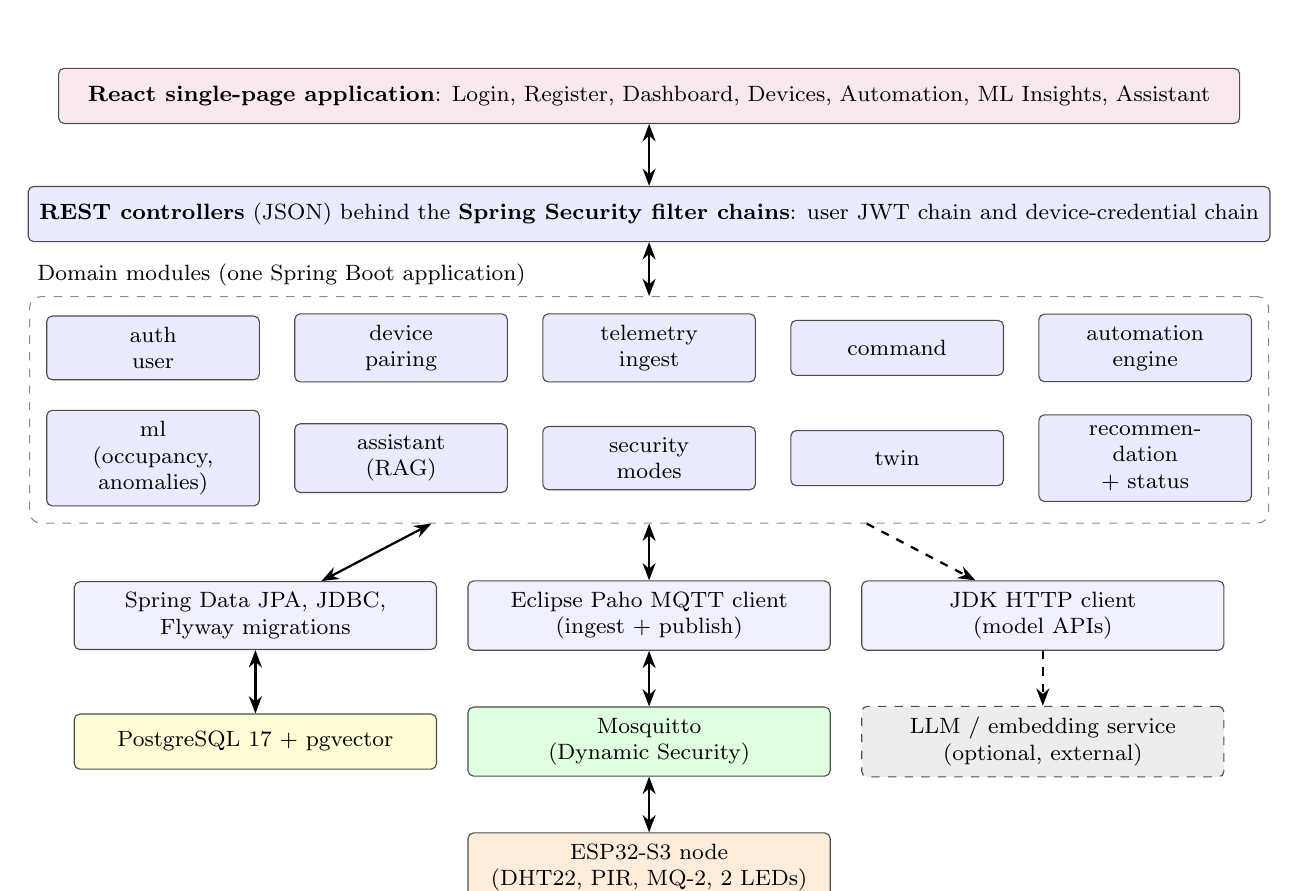
\begin{tikzpicture}[node distance=5mm]
  % presentation
  \node[ui, minimum width=15cm] (ui) at (0,0) {\textbf{React single-page application}: Login, Register, Dashboard, Devices, Automation, ML Insights, Assistant};
  % api
  \node[svc, minimum width=15cm] (api) at (0,-1.5) {\textbf{REST controllers} (JSON) behind the \textbf{Spring Security filter chains}: user JWT chain and device-credential chain};
  % modules
  \node[svc, minimum width=2.7cm] (m1) at (-6.3,-3.2) {auth\\user};
  \node[svc, minimum width=2.7cm] (m2) at (-3.15,-3.2) {device\\pairing};
  \node[svc, minimum width=2.7cm] (m3) at (0,-3.2) {telemetry\\ingest};
  \node[svc, minimum width=2.7cm] (m4) at (3.15,-3.2) {command};
  \node[svc, minimum width=2.7cm] (m5) at (6.3,-3.2) {automation\\engine};
  \node[svc, minimum width=2.7cm] (m6) at (-6.3,-4.6) {ml\\(occupancy,\\anomalies)};
  \node[svc, minimum width=2.7cm] (m7) at (-3.15,-4.6) {assistant\\(RAG)};
  \node[svc, minimum width=2.7cm] (m8) at (0,-4.6) {security\\modes};
  \node[svc, minimum width=2.7cm] (m9) at (3.15,-4.6) {twin};
  \node[svc, minimum width=2.7cm] (m10) at (6.3,-4.6) {recommen-\\dation\\+ status};
  \node[group, fit=(m1)(m2)(m3)(m4)(m5)(m6)(m7)(m8)(m9)(m10), label={[font=\footnotesize]above left:Domain modules (one Spring Boot application)}] (dom) {};
  % infrastructure
  \node[box, minimum width=4.6cm] (jpa) at (-5,-6.6) {Spring Data JPA, JDBC,\\Flyway migrations};
  \node[box, minimum width=4.6cm] (paho) at (0,-6.6) {Eclipse Paho MQTT client\\(ingest + publish)};
  \node[box, minimum width=4.6cm] (http) at (5,-6.6) {JDK HTTP client\\(model APIs)};
  % external
  \node[store, minimum width=4.6cm] (pg) at (-5,-8.2) {PostgreSQL 17 + pgvector};
  \node[broker, minimum width=4.6cm] (mos) at (0,-8.2) {Mosquitto\\(Dynamic Security)};
  \node[ext, minimum width=4.6cm] (llm) at (5,-8.2) {LLM / embedding service\\(optional, external)};
  \node[dev, minimum width=4.6cm] (esp) at (0,-9.8) {ESP32-S3 node\\(DHT22, PIR, MQ-2, 2 LEDs)};
  \draw[<->, thick] (ui) -- (api);
  \draw[<->, thick] (api) -- (dom);
  \draw[<->, thick] (dom) -- (jpa);
  \draw[<->, thick] (dom) -- (paho);
  \draw[->, thick, dashed] (dom) -- (http);
  \draw[<->, thick] (jpa) -- (pg);
  \draw[<->, thick] (paho) -- (mos);
  \draw[->, thick, dashed] (http) -- (llm);
  \draw[<->, thick] (mos) -- (esp);
\end{tikzpicture}}
\caption{Layered architecture. Dashed arrows are optional links.}
\label{fig:layers}
\end{figure}

\section{Deployment View}
Everything runs on one machine on the home network (Figure~\ref{fig:deploy}). PostgreSQL and Mosquitto run in Docker containers started by Docker Compose; the backend and the frontend development server run directly on the host. The ESP32 reaches the backend (for pairing only) and the broker over the local Wi-Fi using the host's LAN address.

\begin{figure}[H]
\centering
\resizebox{0.95\textwidth}{!}{%
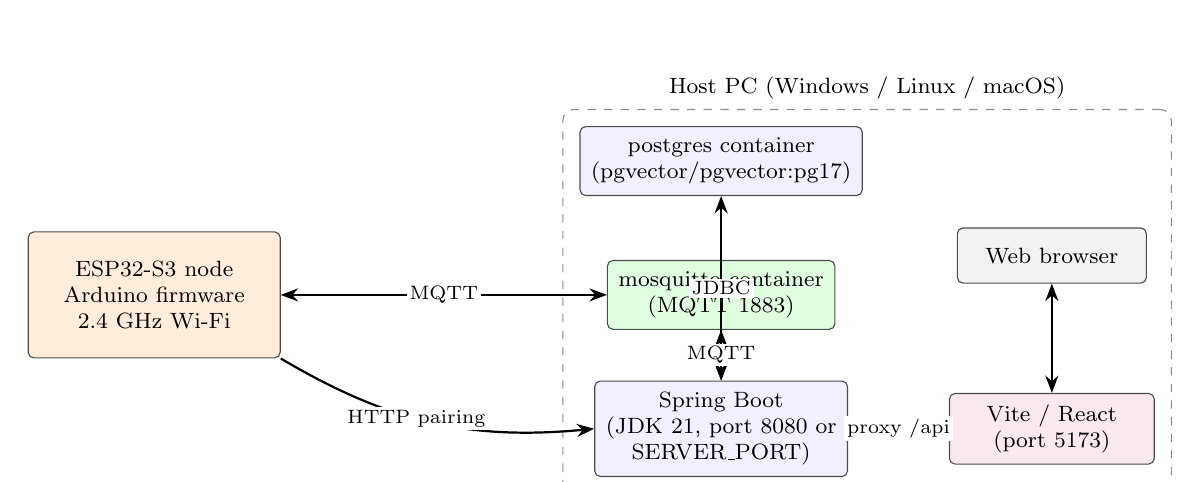
\begin{tikzpicture}
  \node[dev, minimum width=3.2cm, minimum height=1.6cm] (esp) at (0,0) {ESP32-S3 node\\Arduino firmware\\2.4~GHz Wi-Fi};
  \node[box, minimum width=2.6cm] (pg) at (7.2,1.7) {postgres container\\(pgvector/pgvector:pg17)};
  \node[box, minimum width=2.6cm, fill=green!12] (mq) at (7.2,0) {mosquitto container\\(MQTT 1883)};
  \node[box, minimum width=2.6cm] (be) at (7.2,-1.7) {Spring Boot\\(JDK 21, port 8080 or\\SERVER\_PORT)};
  \node[box, minimum width=2.6cm, fill=purple!9] (fe) at (11.4,-1.7) {Vite / React\\(port 5173)};
  \node[box, minimum width=2.4cm, fill=gray!10] (br) at (11.4,0.5) {Web browser};
  \node[group, fit=(pg)(mq)(be)(fe), label={[font=\footnotesize]above:Host PC (Windows / Linux / macOS)}] (host) {};
  \draw[<->, thick] (esp) -- node[lbl]{MQTT} (mq);
  \draw[->, thick] (esp.south east) to[bend right=18] node[lbl, pos=0.45]{HTTP pairing} (be.west);
  \draw[<->, thick] (be) -- node[lbl]{JDBC} (pg);
  \draw[<->, thick] (be) -- node[lbl]{MQTT} (mq);
  \draw[<->, thick] (fe) -- node[lbl]{proxy /api} (be);
  \draw[<->, thick] (br) -- (fe);
\end{tikzpicture}}
\caption{Deployment of the prototype on a single host.}
\label{fig:deploy}
\end{figure}

\section{Backend Module Map}
Table~\ref{tab:modules} lists the Java packages under \code{com.smarthome} and their responsibilities. The backend contains 170 Java source files and the test tree 40.

\begin{table}[H]
\centering
\caption{Backend packages}
\label{tab:modules}
\begin{tabularx}{\textwidth}{lX}
\toprule
\textbf{Package} & \textbf{Responsibility}\\
\midrule
\code{auth}, \code{user} & Registration, login, JWT issuing, profile; BCrypt password hashing.\\
\code{device} & Devices, pairing codes, ownership, presence (online/offline/never connected), device-credential authentication, disown.\\
\code{telemetry} & MQTT message validation, de-duplication, storage, events published after commit.\\
\code{command} & Command allow-list, creation, delivery, acknowledgement, reported LED state, lifecycle sweeper.\\
\code{mqtt} & Paho client, Mosquitto Dynamic Security administration, publisher abstraction.\\
\code{automation} & Rules, validator, condition evaluator, engine, scheduler, execution history.\\
\code{ml} & Occupancy model (logistic regression), anomaly detectors, scanner, trainers, schedulers.\\
\code{assistant} & Chunking, embeddings, pgvector store, indexer, prompt builder, grounding check, model clients, chat and suggestions.\\
\code{security} & Away/Night modes, security events, offline watcher.\\
\code{twin} & Digital twin computation (confirmed versus reported state).\\
\code{recommendation} & Evidence-based recommendations with approval.\\
\code{health} & Public liveness endpoint and the authenticated system-status service.\\
\code{config} & Security filter chains, CORS, exception-to-HTTP mapping, shared configuration.\\
\bottomrule
\end{tabularx}
\end{table}

\section{Messaging Architecture}
\subsection{MQTT topics and access control}
All device traffic uses MQTT 3.1.1 on topics under \texttt{home/devices/\{deviceId\}/}. The broker has anonymous access disabled and uses the Dynamic Security plugin: the backend creates one account per paired device and removes it when the device is disowned. Table~\ref{tab:topics} lists the topics.

\begin{table}[H]
\centering
\caption{MQTT topics (verified against the README and the backend code)}
\label{tab:topics}
\begin{tabularx}{\textwidth}{llX}
\toprule
\textbf{Topic suffix} & \textbf{Direction} & \textbf{Purpose and delivery}\\
\midrule
\code{telemetry} & device $\to$ backend & Sensor readings; not retained.\\
\code{status} & device $\to$ backend & \texttt{\{"state":"online"\}} after connecting (retained, QoS~1); Last Will \texttt{\{"state":"offline"\}}.\\
\code{commands} & backend $\to$ device & One command; QoS~1, never retained. Only the backend account may publish; a device may subscribe only to its own.\\
\code{acks} & device $\to$ backend & The device's answer to a command.\\
\code{state} & device $\to$ backend & What the LEDs are actually doing (not retained).\\
\bottomrule
\end{tabularx}
\end{table}

\subsection{Telemetry data flow}
Figure~\ref{fig:telemetry-flow} follows one reading from the sensor to the screens and background consumers. Identity always comes from the topic and the authenticated broker connection, never from the payload.

\begin{figure}[H]
\centering
\resizebox{\textwidth}{!}{%
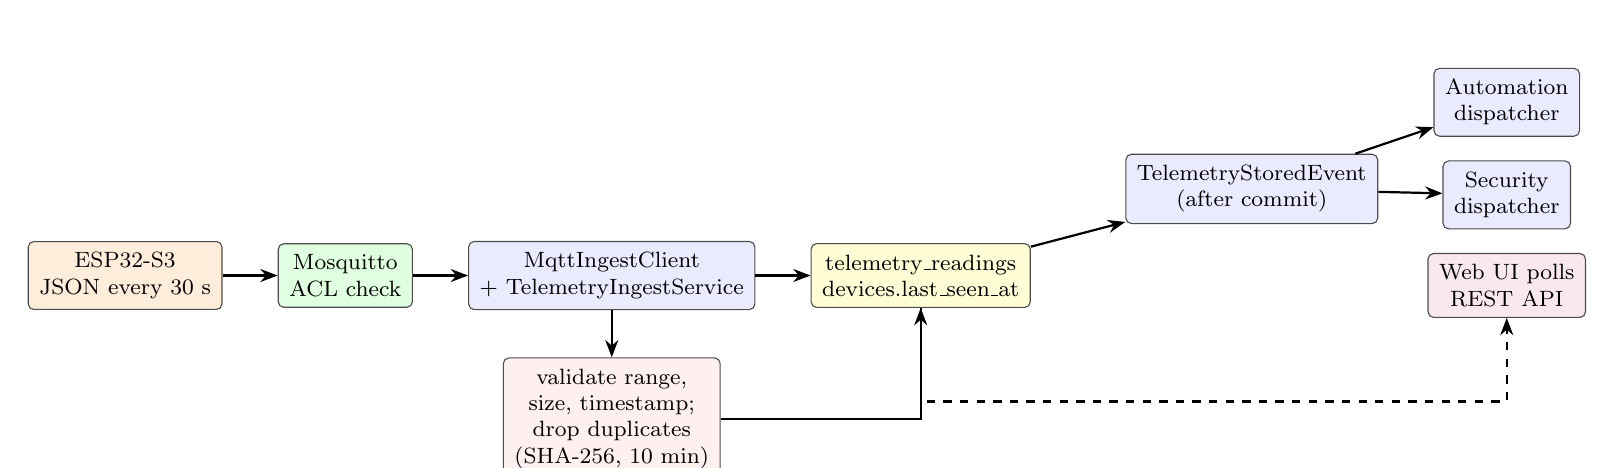
\begin{tikzpicture}[node distance=6mm and 7mm]
  \node[dev] (d) {ESP32-S3\\JSON every 30~s};
  \node[broker, right=of d] (b) {Mosquitto\\ACL check};
  \node[svc, right=of b] (i) {MqttIngestClient\\+ TelemetryIngestService};
  \node[box, below=of i, fill=red!6] (v) {validate range,\\size, timestamp;\\drop duplicates\\(SHA-256, 10 min)};
  \node[store, right=of i] (db) {telemetry\_readings\\devices.last\_seen\_at};
  \node[svc, right=12mm of db, yshift=11mm] (ev) {TelemetryStoredEvent\\(after commit)};
  \node[svc, right=of ev, yshift=11mm] (a) {Automation\\dispatcher};
  \node[svc, below=3mm of a] (s) {Security\\dispatcher};
  \node[ui, below=3mm of s] (u) {Web UI polls\\REST API};
  \draw[flow] (d) -- (b);
  \draw[flow] (b) -- (i);
  \draw[flow] (i) -- (v);
  \draw[flow] (v) -| (db);
  \draw[flow] (i) -- (db);
  \draw[flow] (db) -- (ev);
  \draw[flow] (ev) -- (a);
  \draw[flow] (ev) -- (s);
  \draw[flow, dashed] (db) -- ++(0,-1.6) -| (u);
\end{tikzpicture}}
\caption{Telemetry data flow. Rejected messages are logged by reason only (never the payload).}
\label{fig:telemetry-flow}
\end{figure}

An important implementation detail: work triggered by a stored reading (rule evaluation, security checks) is handed to a dedicated single worker thread \emph{after} the database transaction commits. Calling repositories from inside an \code{AFTER_COMMIT} callback silently joins the already finished transaction and loses writes; the dedicated worker avoids that and also keeps command publishing off the MQTT callback thread.

\subsection{Command data flow}
Figure~\ref{fig:command-seq} shows a remote command. The same path is used by people, automation rules and security modes; only the recorded origin differs.

\begin{figure}[H]
\centering
\resizebox{\textwidth}{!}{%
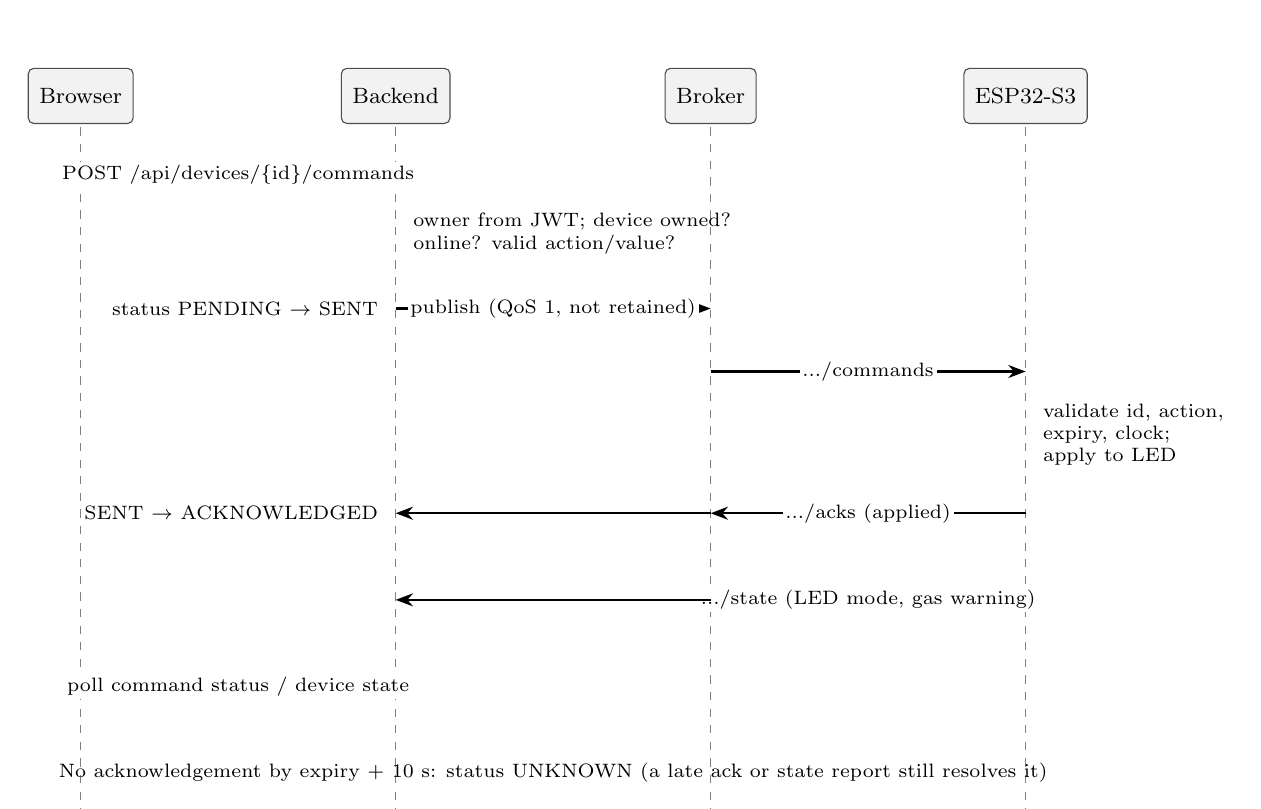
\begin{tikzpicture}[x=1cm,y=1cm]
  \foreach \x/\n in {0/Browser, 4/Backend, 8/Broker, 12/ESP32-S3}{
    \node[box, fill=gray!10] at (\x,0) {\n};
    \draw[dashed, black!50] (\x,-0.4) -- (\x,-9.2);
  }
  \draw[->, thick] (0,-1.0) -- node[lbl]{POST /api/devices/\{id\}/commands} (4,-1.0);
  \node[font=\scriptsize, align=left, anchor=west] at (4.1,-1.75) {owner from JWT; device owned?\\online? valid action/value?};
  \draw[->, thick] (4,-2.7) -- node[lbl]{publish (QoS 1, not retained)} (8,-2.7);
  \node[font=\scriptsize, anchor=east] at (3.9,-2.7) {status PENDING $\to$ SENT};
  \draw[->, thick] (8,-3.5) -- node[lbl]{.../commands} (12,-3.5);
  \node[font=\scriptsize, align=left, anchor=west] at (12.1,-4.3) {validate id, action,\\expiry, clock;\\apply to LED};
  \draw[->, thick] (12,-5.3) -- node[lbl]{.../acks (applied)} (8,-5.3);
  \draw[->, thick] (8,-5.3) -- (4,-5.3);
  \node[font=\scriptsize, anchor=east] at (3.9,-5.3) {SENT $\to$ ACKNOWLEDGED};
  \draw[->, thick] (12,-6.4) -- node[lbl]{.../state (LED mode, gas warning)} (8,-6.4);
  \draw[->, thick] (8,-6.4) -- (4,-6.4);
  \draw[->, thick] (4,-7.5) -- node[lbl]{poll command status / device state} (0,-7.5);
  \node[font=\scriptsize, align=center] at (6,-8.6) {No acknowledgement by expiry + 10~s: status UNKNOWN (a late ack or state report still resolves it)};
\end{tikzpicture}}
\caption{Sequence of a remote LED command.}
\label{fig:command-seq}
\end{figure}

\section{Security Boundaries}
Two independent Spring Security filter chains separate the two kinds of caller. The \emph{device chain} (path \api{/api/device/**}) accepts only device credentials; the \emph{user chain} (everything else) accepts only user JWTs. A user JWT never works on a device endpoint and a device credential never works on a user endpoint. Only \code{POST /api/device/pair} is open on the device chain, because its proof is the one-time pairing code.

% =====================================================================================
%  CHAPTER 5  HARDWARE AND FIRMWARE
% =====================================================================================
\chapter{Hardware Design and Firmware}
\label{ch:hardware}

\begin{center}
\fbox{\parbox{0.93\textwidth}{\small\textbf{Validation status.} The firmware compiles with the ESP32 Arduino core, and its payload builders, pairing-code parser, back-off logic, gas-warning logic and command validation are unit-tested on a PC. Its payload formats and command handling were replayed against the real broker and backend. \textbf{It has not yet been run on a physical ESP32-S3 board}, so the behaviour described in this chapter is the intended and PC-tested behaviour; the hardware verification checklist (Section~\ref{sec:hwchecklist}) is still to be carried out. In addition, the original sketch was not available when the firmware was written, so the LED and gas-warning behaviour was written from scratch.}}
\end{center}

\section{Components}
Table~\ref{tab:components} lists the parts of the sensor node.
\begin{table}[H]
\centering
\caption{Sensor node components}
\label{tab:components}
\begin{tabularx}{\textwidth}{lX}
\toprule
\textbf{Component} & \textbf{Role in the system}\\
\midrule
ESP32-S3 development board~\cite{esp32s3} & Microcontroller with Wi-Fi (2.4~GHz only); runs the firmware (Arduino framework, C++).\\
DHT22~\cite{dht22} & Digital temperature and relative-humidity sensor on one data pin. Needs at least 2~s between reads.\\
PIR motion sensor module & Digital output that goes high when motion is seen. Its output level must be 3.3~V.\\
MQ-2 gas sensor module & Analog output (AO) read by the ESP32 ADC (12-bit, counts 0--4095). The value is kept as a \emph{raw ADC count}; it is never converted to ppm because that would need calibration which was not performed.\\
LED (PIR indicator) & Lights while motion is detected, or as commanded.\\
LED (gas warning) & Lights during a gas warning, or when forced on for identification.\\
Resistors & About 220--330~$\Omega$ in series with each LED; about 10~k$\Omega$ pull-up on the DHT22 data line; optional 10~k$\Omega$ + 20~k$\Omega$ divider on the MQ-2 AO line.\\
\bottomrule
\end{tabularx}
\end{table}

\section{Pin Assignment}
Table~\ref{tab:pins} gives the pins defined in \code{config.h}. Two assignments differ from the original specification because the original GPIO numbers cannot work on an ESP32-S3: GPIO35 has no ADC (the ADC inputs of the S3 are GPIO1--20; GPIO4 is ADC1 channel~3), and GPIO26 is connected to the module's flash/PSRAM (GPIO26--37 are reserved on common S3 modules). The firmware refuses to build if a pin is unsuitable for the S3.

\begin{table}[H]
\centering
\caption{GPIO assignment (from the firmware configuration header)}
\label{tab:pins}
\begin{tabularx}{\textwidth}{llX}
\toprule
\textbf{Function} & \textbf{GPIO} & \textbf{Note}\\
\midrule
DHT22 data & 14 & As originally specified.\\
PIR output & 5 & Moved from 26 (flash/PSRAM range on the S3).\\
PIR indicator LED & 12 & As originally specified.\\
MQ-2 analog output (AO) & 4 & Moved from 35 (no ADC on the S3); ADC1 channel~3.\\
Gas warning LED & 13 & As originally specified.\\
\bottomrule
\end{tabularx}
\end{table}

\section{Wiring Diagram}
Figure~\ref{fig:wiring} shows the connections. The MQ-2 module's analog output can reach 5~V when the module is powered from 5~V, which can damage the ESP32-S3 (its pins tolerate 3.3~V only). The module should therefore be powered from 3.3~V, or a voltage divider should be placed between AO and GPIO4.

\begin{figure}[H]
\centering
\resizebox{0.98\textwidth}{!}{%
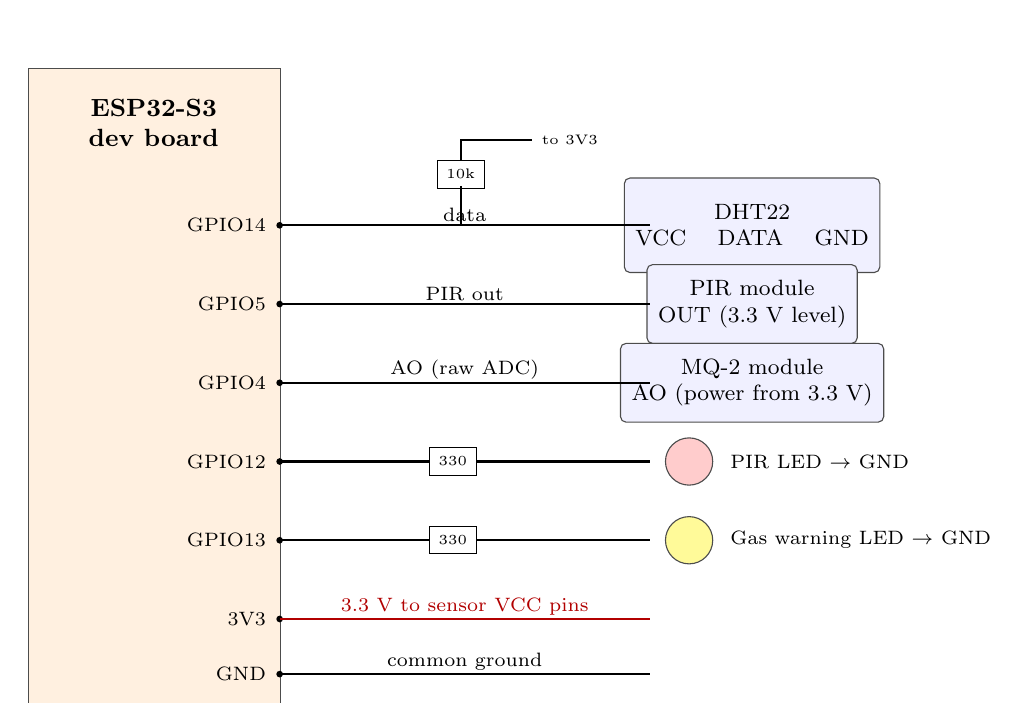
\begin{tikzpicture}[x=1cm,y=1cm]
  % ESP32 board
  \node[draw=black!70, fill=orange!12, minimum width=3.2cm, minimum height=8.2cm, anchor=north west, align=center] (mcu) at (0,0) {};
  \node[font=\small\bfseries, align=center] at (1.6,-0.7) {ESP32-S3\\dev board};
  \foreach \y/\p in {-2.0/GPIO14, -3.0/GPIO5, -4.0/GPIO4, -5.0/GPIO12, -6.0/GPIO13, -7.0/3V3, -7.7/GND}{
    \node[font=\scriptsize, anchor=east] at (3.15,\y) {\p};
    \fill (3.2,\y) circle (1.2pt);
  }
  % DHT22
  \node[box, minimum width=2.6cm, minimum height=1.2cm] (dht) at (9.2,-2.0) {DHT22\\VCC \quad DATA \quad GND};
  \draw[thick] (3.2,-2.0) -- node[lbl, above]{data} (7.9,-2.0);
  \node[draw, minimum width=6mm, minimum height=2.5mm, fill=white, font=\tiny] (pu) at (5.5,-1.35) {10k};
  \draw[thick] (5.5,-1.5) -- (5.5,-2.0);
  \draw[thick] (pu.north) -- ++(0,0.25) -- ++(0.9,0) node[font=\tiny, right]{to 3V3};
  % PIR
  \node[box, minimum width=2.6cm, minimum height=1.0cm] (pir) at (9.2,-3.0) {PIR module\\OUT (3.3 V level)};
  \draw[thick] (3.2,-3.0) -- node[lbl, above]{PIR out} (7.9,-3.0);
  % MQ-2
  \node[box, minimum width=2.6cm, minimum height=1.0cm] (mq) at (9.2,-4.0) {MQ-2 module\\AO (power from 3.3 V)};
  \draw[thick] (3.2,-4.0) -- node[lbl, above]{AO (raw ADC)} (7.9,-4.0);
  % LEDs
  \node[draw, minimum width=6mm, minimum height=2.5mm, fill=white, font=\tiny] (r1) at (5.4,-5.0) {330};
  \draw[thick] (3.2,-5.0) -- (r1.west);
  \draw[thick] (r1.east) -- (7.9,-5.0);
  \node[draw=black!70, circle, fill=red!20, minimum size=6mm, font=\scriptsize] (led1) at (8.4,-5.0) {};
  \node[font=\scriptsize, anchor=west] at (8.8,-5.0) {PIR LED $\to$ GND};
  \node[draw, minimum width=6mm, minimum height=2.5mm, fill=white, font=\tiny] (r2) at (5.4,-6.0) {330};
  \draw[thick] (3.2,-6.0) -- (r2.west);
  \draw[thick] (r2.east) -- (7.9,-6.0);
  \node[draw=black!70, circle, fill=yellow!40, minimum size=6mm, font=\scriptsize] (led2) at (8.4,-6.0) {};
  \node[font=\scriptsize, anchor=west] at (8.8,-6.0) {Gas warning LED $\to$ GND};
  % power
  \draw[thick, red!70!black] (3.2,-7.0) -- node[lbl, above]{3.3 V to sensor VCC pins} (7.9,-7.0);
  \draw[thick, black] (3.2,-7.7) -- node[lbl, above]{common ground} (7.9,-7.7);
\end{tikzpicture}}
\caption{Wiring of the sensor node (schematic). Resistor values are the typical ranges given in the README; check the datasheets of the modules actually used.}
\label{fig:wiring}
\end{figure}

\section{Firmware Structure}
The firmware (directory \code{firmware/smarthome_esp32s3}) is split (Table~\ref{tab:fwfiles}) so that the safety-relevant logic can be tested on a PC without hardware.
\begin{table}[H]
\centering
\caption{Firmware files}
\label{tab:fwfiles}
\begin{tabularx}{\textwidth}{lX}
\toprule
\textbf{File} & \textbf{Content}\\
\midrule
\code{config.h} & Pins, timings, gas thresholds, limits, topic prefix; compile-time checks that pins suit the S3.\\
\code{Logic.h} & Pure logic (no hardware calls): payload building, gas hysteresis, LED mode resolution, back-off, pairing-code parsing. Unit-tested on a PC.\\
\code{CommandParser.h} & Validation of a command message (UUID id, allow-listed action and value, expiry rules).\\
\code{Sensors.cpp/.h} & PIR polling, DHT22 reads, MQ-2 sampling and averaging.\\
\code{NetLink.cpp/.h} & Wi-Fi, NTP, pairing over HTTP, MQTT connection, publishing, command handling (runs on the second core).\\
\code{secrets.example.h} & Template for the private \code{secrets.h} (Wi-Fi and server addresses); the real file is git-ignored.\\
\bottomrule
\end{tabularx}
\end{table}

The sensing loop and the networking task run on different cores, so slow or failed network connections never stall the sensors or the LEDs.

\section{Local Behaviour that Needs No Network}
\subsection{PIR indicator LED}
The PIR input is polled every 20~ms and the PIR LED follows it immediately.

\subsection{Gas warning with hysteresis}
The MQ-2 is sampled every 250~ms and a moving average of 8 raw counts is kept. During the first 60~s the heater is warming up: no warning is raised and no gas value is published. Afterwards the warning state uses hysteresis so that it does not flicker around a single threshold (Figure~\ref{fig:gas-states}). The thresholds in \code{config.h} are \textbf{placeholders} (warn at 2000 counts, clear below 1800) and must be calibrated against the real sensor in clean air and with a gas source before any reliance.

\begin{figure}[H]
\centering
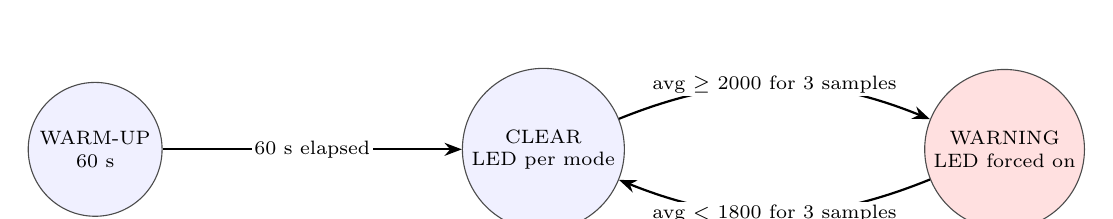
\begin{tikzpicture}[node distance=38mm]
  \node[state, minimum size=17mm] (w) {WARM-UP\\60 s};
  \node[state, minimum size=17mm, right=of w] (c) {CLEAR\\LED per mode};
  \node[state, minimum size=17mm, fill=red!12, right=of c] (a) {WARNING\\LED forced on};
  \draw[->, thick] (w) -- node[lbl]{60 s elapsed} (c);
  \draw[->, thick] (c) to[bend left=22] node[lbl]{avg $\ge$ 2000 for 3 samples} (a);
  \draw[->, thick] (a) to[bend left=22] node[lbl]{avg $<$ 1800 for 3 samples} (c);
\end{tikzpicture}
\caption{Gas warning states. Remote commands never read or change this logic.}
\label{fig:gas-states}
\end{figure}

\subsection{Remote LED modes}
Table~\ref{tab:ledmodes} lists what remote commands can change.
\begin{table}[H]
\centering
\caption{LED modes (allow-list shared by the backend and the firmware)}
\label{tab:ledmodes}
\begin{tabularx}{\textwidth}{llX}
\toprule
\textbf{Action} & \textbf{Values} & \textbf{Effect}\\
\midrule
\code{set_pir_led} & auto, on, off & auto: follows motion; on: forced lit; off: forced unlit.\\
\code{set_gas_led} & auto, on & auto: shows the gas warning; on: forced lit to identify the device. There is deliberately no ``off''.\\
\bottomrule
\end{tabularx}
\end{table}
A forced mode returns to \emph{auto} after one hour and on reboot. The gas LED is always lit during a gas warning, whatever mode is set, and \code{set_gas_led} with \code{off} is refused.

\section{Networking, Presence and Telemetry}
Wi-Fi reconnection uses exponential back-off from 1~s to 60~s, MQTT from 2~s to 120~s, both with 20\% jitter and reset on success. The MQTT connection uses the device identifier as the user name and the stored credential as the password, a Last Will of \texttt{\{"state":"offline"\}} (retained), and publishes \texttt{\{"state":"online"\}} after connecting. Every 30~s the node publishes a telemetry message (Listing~\ref{lst:telemetry}); \code{seq} always increases, also across reboots; \code{ts} is sent only after NTP has set the clock; the DHT22 values are omitted if the last good read is older than 15~s; \code{motion} is true if motion occurred at any time since the previous report; \code{gasRaw} is omitted while warming up.

\begin{lstlisting}[caption={Telemetry payload (maximum 1024 bytes; at least one reading is required)},label={lst:telemetry}]
{ "seq": 42, "ts": 1792830977, "temperature": 24.5,
  "humidity": 55.2, "motion": true, "gasRaw": 1834 }
\end{lstlisting}

\section{Pairing and Credential Storage}
Figure~\ref{fig:pairing} shows the pairing sequence.
\begin{figure}[H]
\centering
\resizebox{\textwidth}{!}{%
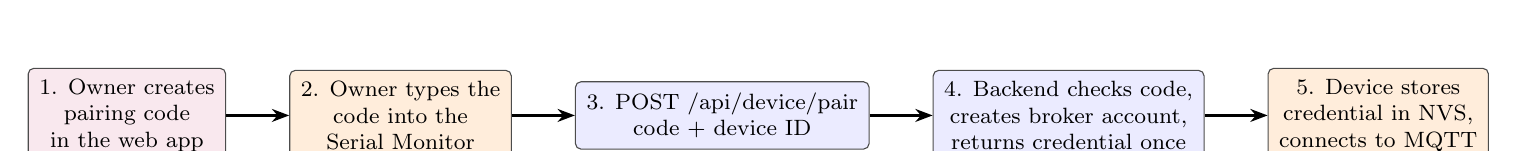
\begin{tikzpicture}[node distance=7mm and 8mm]
  \node[ui] (a) {1. Owner creates\\pairing code\\in the web app};
  \node[dev, right=of a] (b) {2. Owner types the\\code into the\\Serial Monitor};
  \node[svc, right=of b] (c) {3. POST /api/device/pair\\code + device ID};
  \node[svc, right=of c] (d) {4. Backend checks code,\\creates broker account,\\returns credential once};
  \node[dev, right=of d] (e) {5. Device stores\\credential in NVS,\\connects to MQTT};
  \draw[flow] (a) -- (b); \draw[flow] (b) -- (c); \draw[flow] (c) -- (d); \draw[flow] (d) -- (e);
\end{tikzpicture}}
\caption{Device pairing flow. A hardware identifier or MAC address alone never claims a device.}
\label{fig:pairing}
\end{figure}
The device identifier is \code{esp32-} followed by the Wi-Fi MAC address; it only names the device. The credential is stored in flash (NVS) and is never printed or logged. Flash is not encrypted by default, so someone with physical access to the board could read it; flash encryption is recommended beyond a college demonstration. Serial commands (local USB only) are the pairing code itself, \code{status}, \code{reset} and \code{help}.

\section{Hardware Verification Checklist (Pending)}
\label{sec:hwchecklist}
The README contains a fourteen-step checklist for the physical board; \textbf{none of these steps has been performed yet}. In summary, they check: sensing with no network; DHT22 and MQ-2 readings and calibration of the gas thresholds; pairing; correct data on the web page; behaviour when the network or broker disappears; the Last Will; reboot behaviour; disowning; the PIR and gas LED commands; and that the gas warning cannot be suppressed by any command.

% =====================================================================================
%  CHAPTER 6  TECHNOLOGY STACK
% =====================================================================================
\chapter{Technology Stack}
\label{ch:tech}

Table~\ref{tab:stack} lists the technologies used, with the versions found in the build files and the README.

\begin{table}[H]
\centering
\caption{Technologies and versions (taken from the project's build files and README)}
\label{tab:stack}
\begin{tabularx}{\textwidth}{lXl}
\toprule
\textbf{Layer} & \textbf{Technology and purpose} & \textbf{Version}\\
\midrule
Language & Java (backend) & 21\\
Framework & Spring Boot: web MVC, security, OAuth2 resource server (JWT), data JPA, validation, Flyway & 4.1.1\\
Build & Maven (bundled wrapper) & wrapper\\
Database & PostgreSQL with the pgvector extension (Docker image \code{pgvector/pgvector:pg17}) & 17\\
Migrations & Flyway; vendor-specific folder for the vector column & --\\
Messaging & Eclipse Mosquitto with the Dynamic Security plugin; Eclipse Paho MQTT v3 client & Mosquitto 2.x\\
Tokens & HS256 JSON Web Tokens (Nimbus via Spring Security); BCrypt password hashing & --\\
JSON & Jackson (Spring Boot 4 uses Jackson 3, package \code{tools.jackson}) & --\\
HTTP to models & JDK \code{java.net.http.HttpClient} (no extra dependency) & JDK 21\\
Tests (backend) & JUnit 5, Spring Boot test and MockMvc, H2 in PostgreSQL mode & --\\
Frontend & React, TypeScript, Vite, Tailwind CSS, React Router & React 19, Vite 8, Tailwind 4\\
Frontend quality & TypeScript compiler (\code{tsc -b}), oxlint & --\\
Firmware & Arduino framework for ESP32 (\code{esp32:esp32} core), DHT sensor library, Adafruit Unified Sensor, PubSubClient, ArduinoJson & core 3.3.12; 1.4.7; 1.1.15; 2.8; 7.4.3\\
Packaging & Docker Compose for PostgreSQL and Mosquitto & --\\
\bottomrule
\end{tabularx}
\end{table}

\section{Why These Choices}
\begin{itemize}
  \item \textbf{MQTT} is a lightweight publish/subscribe protocol designed for constrained devices~\cite{mqtt311}; it supports Last Will messages and QoS levels that suit presence detection and command delivery.
  \item \textbf{PostgreSQL with pgvector} lets the relational data and the vector index live in one database, so ownership filters and similarity search happen in the same query~\cite{pgvector}.
  \item \textbf{Spring Boot} provides mature security, validation and persistence components, and the modular-monolith structure fits a single deployable application~\cite{springboot}.
  \item \textbf{Flyway} makes the schema reproducible~\cite{flyway}; Hibernate only validates that the entities match it. PostgreSQL itself is documented in~\cite{postgres}.
  \item \textbf{Mosquitto} is a widely used open-source broker whose Dynamic Security plugin allows per-device accounts and topic permissions to be managed at run time~\cite{mosquitto}.
  \item \textbf{React} with TypeScript gives a typed single-page interface~\cite{react}.
  \item \textbf{Java for machine learning.} The models are small (a logistic regression and robust statistics), so implementing them directly in Java avoids a separate Python service and keeps deployment simple.
\end{itemize}

% =====================================================================================
%  CHAPTER 7  IMPLEMENTED FEATURES
% =====================================================================================
\chapter{Implemented Features (Chunks 1--9)}
\label{ch:features}

This chapter describes what was actually implemented in each increment. Statements are taken from the source code, the migrations, the README and the tests of the project.

% ------------------------------------------------------------------------------------- Chunk 1
\section{Chunk 1: Project Foundation}
The first increment created the skeleton that everything else builds on.
\begin{itemize}
  \item \textbf{Repository layout:} \code{backend/}, \code{frontend/}, \code{firmware/}, \code{infra/}, \code{docker-compose.yml}, \code{.env.example}, \code{.gitignore}.
  \item \textbf{Docker Compose:} a PostgreSQL service using the \code{pgvector/pgvector:pg17} image with a health check, an Eclipse Mosquitto broker, and a one-shot initialisation container that creates the broker's Dynamic Security file with an administrator account only if it does not yet exist. A script in \code{infra/postgres/init/} runs \code{CREATE EXTENSION IF NOT EXISTS vector} on the first start of an empty volume.
  \item \textbf{Configuration without secrets:} all passwords and the JWT secret come from a git-ignored \code{.env} file (a template, \code{.env.example}, contains placeholders only). The backend reads \code{../.env} automatically when started from \code{backend/}. There are no default passwords, and the application refuses to start without a JWT secret of at least 32 characters.
  \item \textbf{Health check:} the public endpoint \api{/api/health} returns the service status; the React application shows it on the dashboard.
\end{itemize}

% ------------------------------------------------------------------------------------- Chunk 2
\section{Chunk 2: Authentication}
\begin{itemize}
  \item \textbf{Endpoints:} \code{POST /api/auth/register}, \code{POST /api/auth/login}, \code{GET /api/auth/me}.
  \item \textbf{Validation:} user names are 3--30 characters from letters, digits, dot, underscore and hyphen; the e-mail address must be valid; passwords are 8--72 characters (BCrypt uses at most the first 72 bytes).
  \item \textbf{Passwords} are stored only as BCrypt hashes~\cite{bcrypt}.
  \item \textbf{Tokens:} on login the backend issues an HS256-signed JWT~\cite{rfc7519} with a fixed issuer and a configurable lifetime (default 60 minutes). The resource-server configuration verifies signature, expiry and issuer on every request. The server is stateless, uses no cookies (so CSRF protection is disabled by design) and allows browser calls only from the configured origins.
  \item \textbf{Frontend:} an authentication context, protected routes that redirect to the login page, and automatic logout when a protected call returns 401. The token is kept in the browser's \code{localStorage}; the source code documents the trade-off that any script running on the page could read it.
\end{itemize}

% ------------------------------------------------------------------------------------- Chunk 3
\section{Chunk 3: Device Registration and Ownership}
\begin{itemize}
  \item \textbf{Pairing codes} are created by a logged-in user (\code{POST /api/devices/pairing-codes}) in a human-friendly format such as \code{ABCD-2345}, are valid for 10 minutes, can be used once, and are stored only as SHA-256 hashes.
  \item \textbf{Claiming:} the device calls \code{POST /api/device/pair} with the code and its hardware identifier and receives a random credential (43 characters) exactly once; only its SHA-256 hash is stored. The owner of the device is whoever created the code; knowing a hardware identifier or MAC address alone can never claim a device.
  \item \textbf{Brute-force protection:} pairing attempts are rate limited per client address.
  \item \textbf{Ownership:} every device query includes the owner's identifier. A device that belongs to someone else, was disowned or does not exist produces the same ``not found'' response, so identifiers cannot be probed.
  \item \textbf{Rename and disown:} disowning revokes the credential, removes the device's account from the broker (which also drops its live connection) and deletes its readings, command history, reported state, rules, models, anomalies, assistant index and security events. If the broker cannot be reached, everything is rolled back and the owner is told to retry, so a device never looks disowned while it can still connect.
\end{itemize}

% ------------------------------------------------------------------------------------- Chunk 4
\section{Chunk 4: MQTT Telemetry and Presence}
The backend runs an MQTT ingest client (Eclipse Paho) that logs in with its own broker account, created automatically on first start together with the broker roles. Each message passes through the checks below before it is stored.
\begin{table}[H]
\centering
\caption{Telemetry validation}
\label{tab:telemetry-rules}
\begin{tabularx}{\textwidth}{lX}
\toprule
\textbf{Field} & \textbf{Rule}\\
\midrule
\code{seq} & Required integer $\ge 0$ that increases per message; also keeps identical readings distinct.\\
\code{ts} & Optional epoch seconds; must be after November 2023 and at most five minutes in the future, otherwise the message is rejected.\\
\code{temperature} & Optional, $-40$ to $125$\,\degC. Omitted when the sensor read failed.\\
\code{humidity} & Optional, 0 to 100\,\%.\\
\code{motion} & Optional boolean (true/false, not 0/1).\\
\code{gasRaw} & Optional integer 0--4095: the raw ADC count, never converted to ppm.\\
\code{deviceId} & If present it must equal the topic's device identifier; identity comes from the topic and the authenticated connection.\\
\bottomrule
\end{tabularx}
\end{table}
Table~\ref{tab:telemetry-rules} summarises the field rules. Further rules: payloads are limited to 1024 bytes; unknown, disowned or invalid devices are ignored; malformed or out-of-range messages are dropped and logged by reason only (never the payload); byte-identical messages within 10 minutes are stored once (QoS~1 redelivery); retained telemetry is ignored; and a value outside its range is also published as an internal event so that the anomaly detector can record it.

\subsection{Presence}
A device is \textbf{ONLINE} only if it reported online \emph{and} the backend received a live message within 90 seconds (configurable). It is \textbf{NEVER\_CONNECTED} until the first live message and \textbf{OFFLINE} if it said so (Last Will) or went silent. Online status is derived from live evidence and is never assumed from a stored row. The user interface marks readings older than the threshold as stale, and a sensor that sent nothing is shown as ``no reading'' instead of zero.

% ------------------------------------------------------------------------------------- Chunk 5
\section{Chunk 5: Secure Remote Commands}
Only the two indicator LEDs can be commanded (Table~\ref{tab:ledmodes}). The allow-list in \code{CommandActions.java} is the single source of truth for validation, the user interface (which renders its buttons from it) and the documentation; the firmware has a matching copy.

\subsection{Command rules}
\begin{itemize}
  \item The owner comes from the JWT; a device that is not yours is ``not found''.
  \item A command is refused with HTTP 409 unless the device is currently ONLINE; nothing is queued for later, so nothing surprising happens when a device reconnects.
  \item An identical command already in flight is returned instead of being sent twice; at most five commands may wait per device (HTTP 429).
  \item Each command has a UUID, an absolute expiry (30~s by default) and is published with QoS~1 and \emph{not} retained. The device refuses a command that is expired, whose expiry is more than ten minutes away, or when its clock is not set.
  \item The device answers on the \code{acks} topic (\code{applied}, \code{rejected} or \code{expired}) and reports the resulting LED state on the \code{state} topic, including the last command identifier so that a lost acknowledgement can be recovered. A device can only resolve its own commands.
  \item The device remembers its last 16 command identifiers: a redelivered command is answered again but never applied twice.
\end{itemize}

\subsection{Command lifecycle}
Figure~\ref{fig:cmd-lifecycle} shows the status transitions of a command.
\begin{figure}[H]
\centering
\resizebox{0.95\textwidth}{!}{%
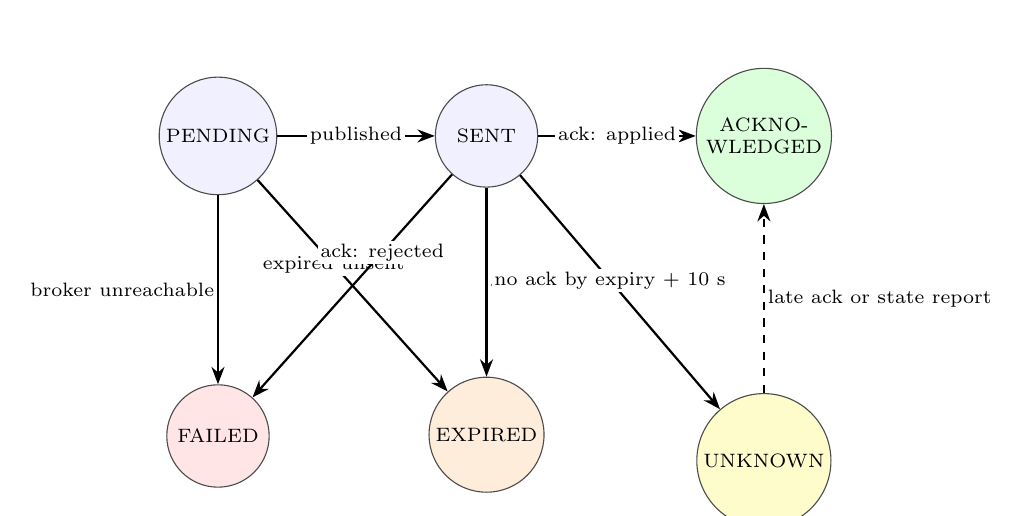
\begin{tikzpicture}[node distance=24mm and 20mm]
  \node[state] (p) {PENDING};
  \node[state, right=of p] (s) {SENT};
  \node[state, right=of s, fill=green!14] (a) {ACKNO-\\WLEDGED};
  \node[state, below=of p, fill=red!10] (f) {FAILED};
  \node[state, below=of s, fill=orange!14] (e) {EXPIRED};
  \node[state, below=of a, fill=yellow!20] (u) {UNKNOWN};
  \draw[->, thick] (p) -- node[lbl]{published} (s);
  \draw[->, thick] (s) -- node[lbl]{ack: applied} (a);
  \draw[->, thick] (p) -- node[lbl, left]{broker unreachable} (f);
  \draw[->, thick] (p) -- node[lbl, pos=0.4]{expired unsent} (e);
  \draw[->, thick] (s) -- node[lbl, pos=0.35]{ack: rejected} (f);
  \draw[->, thick] (s) -- node[lbl, right]{ack: expired} (e);
  \draw[->, thick] (s) -- node[lbl, pos=0.45]{no ack by expiry + 10 s} (u);
  \draw[->, thick, dashed] (u) -- node[lbl, right]{late ack or state report} (a);
\end{tikzpicture}}
\caption{Command status transitions. Every transition is a guarded database update that applies only while the command is still in an allowed source state.}
\label{fig:cmd-lifecycle}
\end{figure}

\subsection{Frontend}
The Devices page shows live readings with freshness, connection state, the LED controls (rendered from the allow-list, so the gas LED has no ``off'' button), what the device itself reports, a gas-warning banner, and the command history with the status of each command.

% ------------------------------------------------------------------------------------- Chunk 6
\section{Chunk 6: Rule-Based Automation Engine}
\subsection{What a rule is}
A rule is plain data: a trigger, a flat list of simple comparisons joined by AND or OR, and one allow-listed LED action. Nothing a user sends is executed as code, SQL or an expression. Listing~\ref{lst:rule} shows a rule.

\begin{lstlisting}[caption={A telemetry rule (from the README)},label={lst:rule}]
{ "name": "Warm room indicator",
  "deviceId": "<UUID of a device you own>",
  "trigger": { "type": "TELEMETRY" },
  "logic": "AND",
  "conditions": [
    { "sensor": "temperature", "operator": ">",  "value": 30 },
    { "sensor": "motion",      "operator": "==", "value": true } ],
  "action": { "action": "set_pir_led", "value": "on" },
  "priority": 20, "cooldownSeconds": 60, "enabled": true }
\end{lstlisting}

\begin{table}[H]
\centering
\caption{Rule fields and limits}
\label{tab:rule-fields}
\begin{tabularx}{\textwidth}{lX}
\toprule
\textbf{Field} & \textbf{Rule}\\
\midrule
\code{trigger.type} & \code{TELEMETRY} (each new valid reading) or \code{SCHEDULE} (a local time of day).\\
Schedule details & Under \code{trigger}: \code{time} in 24-hour \code{HH:mm}; \code{days}, any of MON..SUN; \code{timeZone}, an IANA zone name (offsets such as \code{+05:30} are refused).\\
\code{conditions[]} & Sensor \code{temperature}, \code{humidity}, \code{motion} or \code{gas} (raw); operators $>,\ \ge,\ <,\ \le,\ =,\ \ne$ (motion allows only $=$ and $\ne$); up to 10; a telemetry rule needs at least one.\\
\code{action} & \code{set_pir_led} (auto/on/off) or \code{set_gas_led} (auto/on).\\
\code{priority} & 0--100, default 10; higher wins.\\
\code{cooldownSeconds} & 5--86400, default 60.\\
Limit & At most 50 rules per user.\\
\bottomrule
\end{tabularx}
\end{table}

\subsection{How the engine behaves}
Table~\ref{tab:rule-fields} gives the fields and limits of a rule, and Figure~\ref{fig:automation-flow} shows the main steps of an evaluation.
\begin{itemize}
  \item \textbf{Three-valued conditions.} Each comparison is true, false or \emph{unknown}. An absent reading (sensor failed, MQ-2 warming up) makes it unknown, never zero. A rule acts only when its result is true, so \texttt{temperature < 5 AND motion == true} with no temperature never fires, while the OR version still fires on motion.
  \item \textbf{One command path.} The engine calls the existing command service with the rule owner's identity and the origin ``automation:\emph{rule name}''; ownership, online check, allow-list, expiry and acknowledgement apply exactly as for manual commands.
  \item \textbf{Cooldown} is claimed atomically in the database, so simultaneous evaluations cannot run a rule twice; a run that did not actually happen does not use up the cooldown.
  \item \textbf{Priorities.} Rules competing for the same output of the same device are resolved by highest priority, then oldest rule, then lowest identifier, before cooldowns are considered; the losers are recorded as overridden.
  \item \textbf{Schedules} are evaluated every 15~s in the rule's own time zone, run at most once per local day inside a five-minute window, and a day the backend was not running is recorded as missed instead of running late. Daylight-saving gaps and overlaps follow the JDK rules.
  \item \textbf{Safety.} Switching the gas LED off is refused when a rule is saved, by the command service, and by the engine at run time.
  \item \textbf{Loop and overload protection:} only telemetry triggers rules (never acknowledgements or state reports); at most six automation commands per target device per minute and ten actions per event; a bounded evaluation queue; a per-rule lock; each rule has its own error boundary.
\end{itemize}

\subsection{Audit trail}
Every evaluation that matched or was held back is stored with the sensor values seen, the per-condition results, the outcome, a reason and the command identifier. Identical skips are folded into one row with a repeat count and the latest 200 rows per rule are kept. Table~\ref{tab:outcomes} lists the outcomes.

\begin{table}[H]
\centering
\caption{Automation outcomes}
\label{tab:outcomes}
\begin{tabularx}{\textwidth}{lX}
\toprule
\textbf{Outcome} & \textbf{Meaning}\\
\midrule
\code{EXECUTED} & A command was handed to the command service.\\
\code{FAILED} & The command could not be created or delivered.\\
\code{SKIPPED_COOLDOWN} & Still cooling down.\\
\code{SKIPPED_OFFLINE} & The target device is not online.\\
\code{SKIPPED_NO_DATA} & A needed reading was missing.\\
\code{SKIPPED_STALE_DATA} & The latest reading is too old to act on.\\
\code{SKIPPED_CONFLICT} & A higher-priority rule owns the output.\\
\code{SKIPPED_ALREADY_SET} & The device already reports the requested mode.\\
\code{SKIPPED_RATE_LIMITED} & Too many automation commands for the device.\\
\code{SKIPPED_BUSY} & The same rule was already running.\\
\code{SKIPPED_NOT_OWNED} & The owner no longer owns the target.\\
\code{SKIPPED_UNSAFE} & The action is not allowed (gas LED off).\\
\code{SKIPPED_CONDITIONS_FALSE} & A scheduled rule fired but its conditions were false.\\
\code{SKIPPED_MISSED} & The backend was not running during the window.\\
\bottomrule
\end{tabularx}
\end{table}

\begin{figure}[H]
\centering
\resizebox{\textwidth}{!}{%
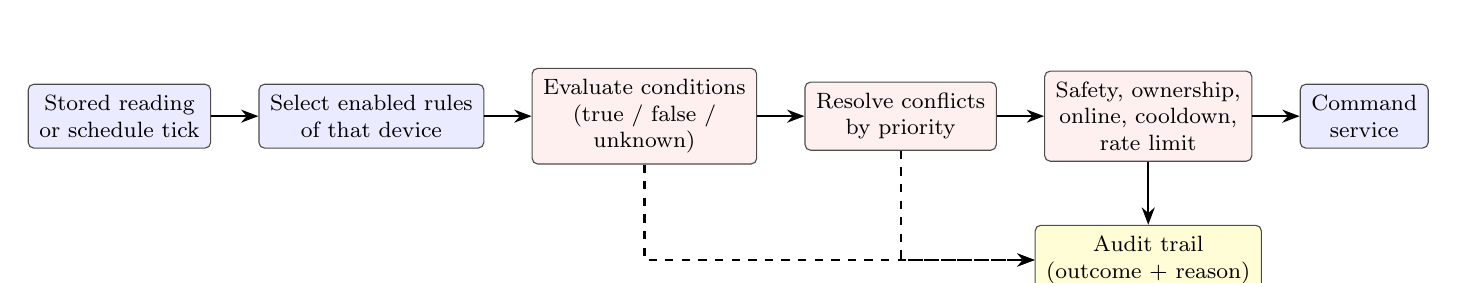
\begin{tikzpicture}[node distance=6mm and 6mm]
  \node[svc] (t) {Stored reading\\or schedule tick};
  \node[svc, right=of t] (r) {Select enabled rules\\of that device};
  \node[box, right=of r, fill=red!6] (c) {Evaluate conditions\\(true / false /\\unknown)};
  \node[box, right=of c, fill=red!6] (k) {Resolve conflicts\\by priority};
  \node[box, right=of k, fill=red!6] (g) {Safety, ownership,\\online, cooldown,\\rate limit};
  \node[svc, right=of g] (cs) {Command\\service};
  \node[store, below=8mm of g] (h) {Audit trail\\(outcome + reason)};
  \draw[flow] (t) -- (r); \draw[flow] (r) -- (c); \draw[flow] (c) -- (k); \draw[flow] (k) -- (g); \draw[flow] (g) -- (cs);
  \draw[flow, dashed] (c) |- (h); \draw[flow, dashed] (k) |- (h); \draw[flow] (g) -- (h);
\end{tikzpicture}}
\caption{Simplified automation flow. The individual checks are listed in Table~\ref{tab:outcomes}; every path ends in an audit record.}
\label{fig:automation-flow}
\end{figure}

\subsection{Frontend}
The Automation page has a rule builder (device to watch and to act on, trigger, conditions, logic, action, priority, cooldown), an enabled switch, edit and delete with confirmation, a per-rule history and a combined recent-activity list with the command status of each run.

% ------------------------------------------------------------------------------------- Chunk 7
\section{Chunk 7: Machine Learning}
Two features were implemented in plain Java (no external ML library): an occupancy predictor and an explainable anomaly detector. The mathematics is given in Chapter~\ref{ch:algorithms}; this section describes the behaviour.

\subsection{Occupancy prediction}
The pipeline is shown in Figure~\ref{fig:ml-pipeline} and the training procedure in Algorithm~\ref{alg:train}.
\begin{itemize}
  \item ``Occupied'' means the PIR sensor fired at least once in a 15-minute slot; it is an activity proxy, not a head count. A slot with fewer than 10 readings is discarded, never treated as ``empty''.
  \item A logistic-regression model is trained on features derived from the time of day and the day of week, and is evaluated on a chronological hold-out set against the baseline of always predicting the training average.
  \item Status values are \code{READY}, \code{LOW_QUALITY} (not better than the baseline, or AUC below 0.6), \code{INSUFFICIENT_DATA} (no model, no metrics, plus the reason) and \code{NOT_TRAINED}. A failed retraining never overwrites a working model.
  \item Training happens only on request (\code{POST .../occupancy/train}, rate limited, one run at a time) or in an hourly check that retrains when at least 24 hours and 1500 new samples have accumulated; never per telemetry message.
  \item Predictions report the probability, the confidence, the number of similar training slots behind the answer (\code{support}) and whether that is reliable.
\end{itemize}

\subsection{Anomaly detection}
Table~\ref{tab:anomaly-kinds} summarises the detectors. Each finding stores a severity, a plain-language explanation and the numbers behind it; one row represents one ongoing problem and counts its occurrences. The scan procedure is given in Algorithm~\ref{alg:scan}.

\begin{table}[H]
\centering
\caption{Anomaly detectors}
\label{tab:anomaly-kinds}
\begin{tabularx}{\textwidth}{lX}
\toprule
\textbf{Kind} & \textbf{Rule (defaults)}\\
\midrule
Statistical outlier & Robust z-score of temperature, humidity or gas against the device's own last 7 days (excluding the last 30 minutes), using the same hour of day $\pm1$\,h when at least 30 samples exist, otherwise all hours; no judgement with fewer than 200 baseline samples. WARNING at $|z|\ge4$, CRITICAL at $|z|\ge6$.\\
Out of range & Temperature outside $-40$ to $80$\,\degC\ (CRITICAL); gas ADC at saturation, 4095 (WARNING). Values rejected by the ingest step are also recorded, escalating to CRITICAL after five occurrences.\\
Stuck value & 60 identical temperature or humidity readings (INFO); 20 identical gas readings (WARNING).\\
Missing data & Ten consecutive messages without temperature/humidity or twenty without gas (WARNING). A missing value is never treated as zero.\\
Stale device & No message for 10 minutes (abandoned after 7 days).\\
\bottomrule
\end{tabularx}
\end{table}
Findings move through the states \code{OPEN}, \code{ACKNOWLEDGED}, \code{RESOLVED}, \code{DISMISSED} and \code{AUTO_RESOLVED}; a dismissed false positive is suppressed for 60 minutes. Scans run about once a minute and on demand. Gas findings carry an advisory note and are never a substitute for the physical alarm.

\begin{figure}[H]
\centering
\resizebox{\textwidth}{!}{%
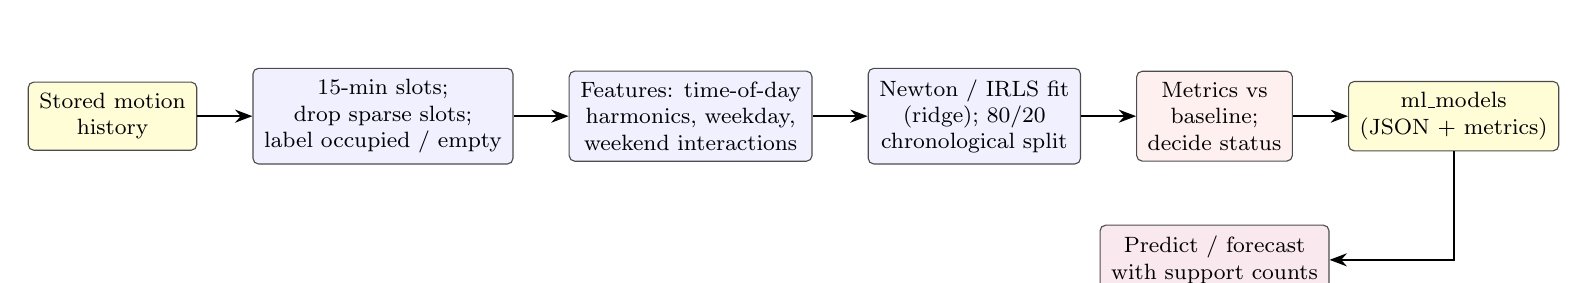
\begin{tikzpicture}[node distance=7mm and 7mm]
  \node[store] (h) {Stored motion\\history};
  \node[box, right=of h] (s) {15-min slots;\\drop sparse slots;\\label occupied / empty};
  \node[box, right=of s] (f) {Features: time-of-day\\harmonics, weekday,\\weekend interactions};
  \node[box, right=of f] (t) {Newton / IRLS fit\\(ridge); 80/20\\chronological split};
  \node[box, right=of t, fill=red!6] (e) {Metrics vs\\baseline;\\decide status};
  \node[store, right=of e] (m) {ml\_models\\(JSON + metrics)};
  \node[ui, below=8mm of e] (p) {Predict / forecast\\with support counts};
  \draw[flow] (h) -- (s); \draw[flow] (s) -- (f); \draw[flow] (f) -- (t); \draw[flow] (t) -- (e); \draw[flow] (e) -- (m); \draw[flow] (m) |- (p);
\end{tikzpicture}}
\caption{Occupancy-model pipeline.}
\label{fig:ml-pipeline}
\end{figure}

\subsection{Frontend}
The ML Insights page shows model readiness with progress towards the required amount of data, a Train button with a time-zone choice, the evaluation metrics next to the baseline, the current prediction, a 24-hour forecast chart with low-evidence hours hatched, and the anomaly list with acknowledge, resolve and dismiss controls, loading, empty and error states.

% ------------------------------------------------------------------------------------- Chunk 8
\section{Chunk 8: AI Assistant with Retrieval-Augmented Generation}
\subsection{Idea}
Retrieval-augmented generation answers a question by first retrieving relevant passages from a knowledge store and then asking a language model to answer \emph{from those passages}~\cite{lewis2020rag}. Here the knowledge store is the user's own data in PostgreSQL, so the assistant can talk about \emph{this} home, not homes in general.

\subsection{Pipeline}
Figure~\ref{fig:rag-pipeline} shows the path of a question and Algorithm~\ref{alg:answer} gives the procedure in steps.
\begin{figure}[H]
\centering
\resizebox{\textwidth}{!}{%
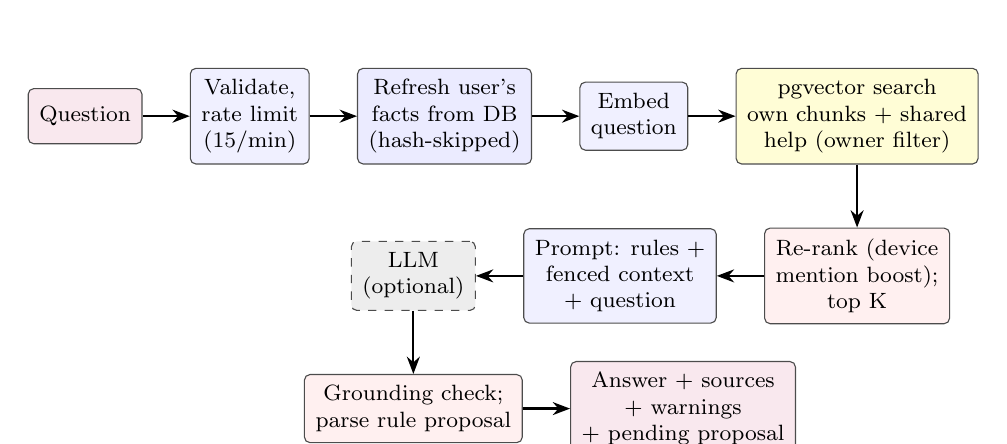
\begin{tikzpicture}[node distance=6mm and 6mm]
  \node[ui] (q) {Question};
  \node[box, right=of q] (v) {Validate,\\rate limit\\(15/min)};
  \node[svc, right=of v] (r) {Refresh user's\\facts from DB\\(hash-skipped)};
  \node[box, right=of r] (em) {Embed\\question};
  \node[store, right=of em] (vs) {pgvector search\\own chunks + shared\\help (owner filter)};
  \node[box, below=8mm of vs, fill=red!6] (rr) {Re-rank (device\\mention boost);\\top K};
  \node[box, left=of rr] (pb) {Prompt: rules +\\fenced context\\+ question};
  \node[ext, left=of pb] (llm) {LLM\\(optional)};
  \node[box, below=8mm of llm, fill=red!6] (gc) {Grounding check;\\parse rule proposal};
  \node[ui, right=of gc] (ans) {Answer + sources\\+ warnings\\+ pending proposal};
  \draw[flow] (q) -- (v); \draw[flow] (v) -- (r); \draw[flow] (r) -- (em); \draw[flow] (em) -- (vs);
  \draw[flow] (vs) -- (rr); \draw[flow] (rr) -- (pb); \draw[flow] (pb) -- (llm);
  \draw[flow] (llm) -- (gc); \draw[flow] (gc) -- (ans);
\end{tikzpicture}}
\caption{Assistant pipeline. If nothing relevant is retrieved the model is not called; if no model is configured the retrieved records are still shown.}
\label{fig:rag-pipeline}
\end{figure}

\subsection{Ingestion (what is indexed)}
Text is split by a chunker into overlapping pieces (about 600 characters with 80 characters of overlap, cut preferably at blank lines, line ends, sentence ends and spaces). Three kinds of text are indexed:
\begin{enumerate}
  \item \textbf{Shared help text} bundled with the application (five Markdown files on sensors, safety, automation, ML insights and devices), indexed once per embedding model with no owner.
  \item \textbf{Live facts} built from the user's real records through the owner-scoped services: device status and latest reading; per-day (UTC, last seven days) and last-24-hour sensor summaries with minimum, average and maximum of the values that exist; anomalies; automation rules and recent runs; ML model state and hold-out metrics. They are rebuilt before a question is answered, at most every 10 seconds per user; unchanged text (SHA-256) is not embedded again and facts whose source disappeared are deleted.
  \item \textbf{User notes}: text the user adds on purpose (20 to 20\,000 characters, up to 20 notes), embedded immediately; nothing is stored if embedding fails.
\end{enumerate}
A missing sensor value is written as ``no value'', and gas is written as a raw value that is not ppm.

\subsection{Embeddings and search}
Two embedding providers are available. The default \textbf{local} embedder is a built-in feature-hashing embedder (256 dimensions, word stems, a small synonym table, sub-linear term weights, identifiers ignored) that needs no network or key; it matches wording, not meaning. The \textbf{openai} provider calls an OpenAI-compatible \code{/embeddings} endpoint (for example a local Ollama server or a hosted service). Chunks record their embedding model, and vectors of different models are never compared; changing the model re-embeds everything.

On PostgreSQL the vector is a pgvector column and the nearest chunks are found with the cosine-distance operator in an exact (not approximate) scan restricted to the caller's own chunks plus the shared help text. On the H2 database used by unit tests the vector is stored as text and the same cosine similarity is computed in Java.

\subsection{Language-model access}
Two real clients exist, both built on the JDK HTTP client: an OpenAI chat-completions client (also used for Ollama, LM Studio and similar servers) and an Anthropic Messages client~\cite{anthropicdocs}. The API key, when needed, is sent only in a request header and is never logged, placed in a prompt or returned by any endpoint. If no provider is configured the assistant still works as a retrieval tool and says so.

\subsection{Safety against hallucination and prompt injection}
The measures below follow the general guidance on prompt injection and over-trusting model output in~\cite{owasp}.
\begin{itemize}
  \item All stored text (device names, notes, rule names, anomaly notes) is treated as \emph{data}: it is placed in a numbered context block delimited by a random per-request token, after the characters \texttt{<<<} and \texttt{>>>} have been neutralised so that stored text cannot close the block or fake a rule proposal. It never appears in the system message.
  \item The system message states that the context is data, that the model cannot control devices, that gas values are raw and that safety must not be asserted.
  \item The answer is checked: citations to sources that do not exist are removed; every number in the answer must appear in the sources (allowing rounding; fractional seconds of timestamps do not count; small whole numbers are exempt); numbers that cannot be found are listed as warnings; an answer with numbers but no citation gets a warning.
  \item If retrieval finds nothing relevant the model is not called and the user is told so.
  \item The model has no tool or code path to devices: it can only produce text. A rule proposal in its reply is parsed, validated with the real rule validator and ownership checks and stored as a \emph{pending} suggestion; it becomes a rule only through an explicit approval, which runs the normal creation service again. A proposal that would switch off the gas LED, or that names another user's device, is discarded with a warning.
\end{itemize}

\subsection{Failure handling}
The answer status tells the user what happened: \code{ANSWERED}, \code{NO_CONTEXT}, \code{NOT_CONFIGURED}, \code{LLM_UNAVAILABLE} (timeout, rejected key, rate limit, server error: the retrieved records are still shown) or \code{RETRIEVAL_UNAVAILABLE} (embedding service down). A database failure returns HTTP 503 with a message that contains no internal detail.

\subsection{Frontend}
The Assistant page offers conversations, example questions, an input with a character counter, answer bubbles with a status badge, amber ``check this'' warnings, a collapsible Sources list (type, text, time, match score; cited sources highlighted), suggestion cards with Approve and Reject, and a notes panel.

% ------------------------------------------------------------------------------------- Chunk 9
\section{Chunk 9: Security Modes, Digital Twin, Recommendations and System Status}
\subsection{Security modes}
The user chooses \textbf{Home} (nothing watched), \textbf{Away} or \textbf{Night}. For Away and Night separately the user configures: whether motion alerts are recorded, the minimum interval between alerts per device (10 to 3600 seconds), and optionally whether the PIR LED is also switched on. The history records mode and settings changes, motion alerts, devices going offline while armed (once per outage) and the LED action taken or failed; alerts can be acknowledged.

\begin{figure}[H]
\centering
\resizebox{\textwidth}{!}{%
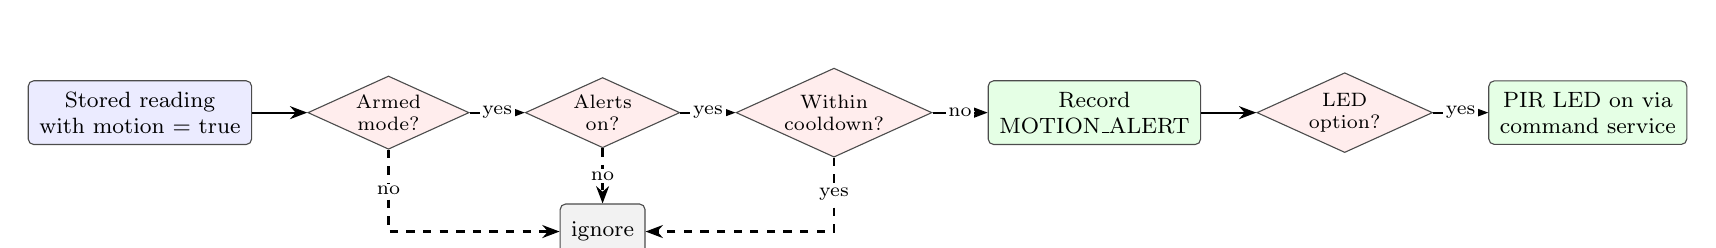
\begin{tikzpicture}[node distance=6mm and 7mm]
  \node[svc] (m) {Stored reading\\with motion = true};
  \node[dec, right=of m] (a) {Armed\\mode?};
  \node[dec, right=of a] (c) {Alerts\\on?};
  \node[dec, right=of c] (r) {Within\\cooldown?};
  \node[box, right=of r, fill=green!10] (e) {Record\\MOTION\_ALERT};
  \node[dec, right=of e] (l) {LED\\option?};
  \node[box, right=of l, fill=green!10] (cs) {PIR LED on via\\command service};
  \node[box, below=7mm of c, fill=gray!10] (ig) {ignore};
  \draw[flow] (m) -- (a);
  \draw[flow] (a) -- node[lbl]{yes} (c);
  \draw[flow] (c) -- node[lbl]{yes} (r);
  \draw[flow] (r) -- node[lbl]{no} (e);
  \draw[flow] (e) -- (l);
  \draw[flow] (l) -- node[lbl]{yes} (cs);
  \draw[flow, dashed] (a) |- node[lbl, pos=0.25]{no} (ig);
  \draw[flow, dashed] (c) -- node[lbl]{no} (ig);
  \draw[flow, dashed] (r) |- node[lbl, pos=0.25]{yes} (ig);
\end{tikzpicture}}
\caption{Handling of a motion reading by the security module.}
\label{fig:security-flow}
\end{figure}

Figure~\ref{fig:security-flow} shows how a motion reading is handled. Properties that matter: (i) the work runs on a dedicated worker thread after the reading is committed, so the cooldown is race-free and nothing runs on the MQTT thread; (ii) telemetry older than two minutes is a replay and never raises an alert; (iii) the LED action goes through the command service with origin \code{security:away} or \code{security:night}; (iv) when the mode ends, a PIR LED that security set is returned to \emph{auto} only if the newest PIR command is still the one security sent, so a value chosen by the owner afterwards is left alone; (v) the only command security can build is \code{set_pir_led}: it never sends a gas-LED command, and changing the mode on its own sends nothing.

\subsection{Device digital twin}
For each output the twin compares the \emph{last confirmed request} (the newest acknowledged command and who asked for it) with what the device \emph{reports}, using only data the existing services already hold. Table~\ref{tab:twin-states} lists the possible states.

\begin{table}[H]
\centering
\caption{Digital-twin synchronisation states}
\label{tab:twin-states}
\begin{tabularx}{\textwidth}{lX}
\toprule
\textbf{State} & \textbf{Condition}\\
\midrule
\code{PENDING} & A command for this output is in flight (pending or sent and not yet expired).\\
\code{NO_DESIRED} & No command was ever acknowledged, so there is nothing to compare.\\
\code{UNREPORTED} & The device has not reported its state recently (or never).\\
\code{UNKNOWN} & A later command was sent but never acknowledged.\\
\code{IN_SYNC} & The reported mode equals the last confirmed request.\\
\code{DRIFT} & The reported mode differs (for example after a restart or a local change).\\
\bottomrule
\end{tabularx}
\end{table}
The twin also reports the connection state, the age of the last contact and of the last reading, pending commands, command problems in the last 24 hours and the gas warning \emph{as the device last reported it}; the warning itself is raised by the firmware.

\subsection{Recommendations}
Three deterministic generators propose changes; each stores its evidence and the exact action approval would take (Table~\ref{tab:recs}). Nothing is applied until the owner approves. Approval calls the normal rule-creation (or rule-disable) service, so ownership, validation and the gas-LED rule are enforced again, and a failed approval leaves the recommendation pending. Dismissed ideas are not offered again for 14 days, applied ones for 30 days, and ideas that stop being valid become stale. When nothing can be suggested the reason is returned as a note (for example ``occupancy model is not trained'').

\begin{table}[H]
\centering
\caption{Recommendation generators}
\label{tab:recs}
\begin{tabularx}{\textwidth}{lXX}
\toprule
\textbf{Generator} & \textbf{Requires} & \textbf{Suggests}\\
\midrule
Quiet hours & Occupancy model in state READY; a run of at least 4 hours in the 24-hour forecast with motion probability below 10\% and enough supporting slots & Two schedule rules: PIR LED off at the start, auto at the end (skipped if such a rule exists)\\
Temperature indicator & At least 3 unusual temperature readings in 7 days and at least 200 stored temperature values & Rule: temperature above the 95th percentile plus 2\,\degC\ turns the PIR LED on, cooldown 5 minutes\\
Failing rules & An enabled rule with at least 5 runs in 7 days of which at least 70\% failed or found the target offline & Disable that rule (it is kept)\\
\bottomrule
\end{tabularx}
\end{table}
Gas readings are never a trigger of a recommendation, and gas is never a target; the PIR LED is used as the indicator because it is the only output a rule may switch back.

\subsection{System status}
One authenticated call, \api{/api/system/status}, reports for the caller's own devices: the database; the MQTT link (connected, disconnected or disabled); each device's availability; command results in the last 24 hours (counts by status, failure rate or ``none sent'', recent problems); per-sensor freshness (fresh, stale or never, only for devices that are online); ML readiness and active anomalies; and the assistant (model configured, search index readable). Every finding is an issue with a level; the overall level (OK, DEGRADED, DOWN) is the worst one, and a check that fails is reported as a problem instead of failing the call. The language model is deliberately \emph{not} called, so ``configured'' does not mean ``reachable''.

\subsection{Frontend}
The dashboard integrates the system-status panel (issues, component states, device and sensor table, command problems), the security panel (mode buttons, configuration, event history with acknowledgement), the recommendations panel (title, rationale, expandable numbers, Approve and Dismiss) and the device-twin panel (confirmed request, reported state, sync badge and notes), each with loading, empty and error states and periodic refresh.

% ------------------------------------------------------------------------------------- Frontend summary
\section{Web Application Summary}
Table~\ref{tab:pages} lists the pages of the web application.
\begin{table}[H]
\centering
\caption{Pages of the React application}
\label{tab:pages}
\begin{tabularx}{\textwidth}{lX}
\toprule
\textbf{Page} & \textbf{Content}\\
\midrule
Login, Register & Forms with server-side field errors.\\
Dashboard & Welcome, system status, security, recommendations, device twins, backend health.\\
Devices & Pairing, device cards with live readings and freshness, LED controls, reported state, command history.\\
Automation & Rule builder, rule list, history.\\
ML Insights & Occupancy readiness, metrics, forecast, anomalies.\\
Assistant & Chat with sources, suggestions, notes.\\
\bottomrule
\end{tabularx}
\end{table}

% =====================================================================================
%  CHAPTER 8  DATABASE DESIGN
% =====================================================================================
\chapter{Database Design}
\label{ch:database}

The schema is created only by Flyway migrations (Table~\ref{tab:migrations}); Hibernate is configured to \emph{validate} that the entities match the schema and never to change it. The database holds 18 tables. Identifiers are UUIDs except for the high-volume telemetry table, which uses a generated 64-bit integer.

\begin{table}[H]
\centering
\caption{Flyway migrations}
\label{tab:migrations}
\begin{tabularx}{\textwidth}{lX}
\toprule
\textbf{Version} & \textbf{Content}\\
\midrule
V1 & \code{users}\\
V2 & \code{devices}, \code{pairing_codes}\\
V3 & Presence columns on \code{devices}; \code{telemetry_readings}\\
V4 & \code{device_commands}, \code{device_reported_state}\\
V5 & \code{automation_rules}, \code{automation_conditions}, \code{automation_executions}; command \code{origin} column\\
V6 & \code{ml_models}, \code{ml_anomalies}\\
V7 & \code{rag_chunks}, \code{chat_conversations}, \code{chat_messages}, \code{assistant_suggestions}\\
V8 & Vendor-specific: on PostgreSQL \code{CREATE EXTENSION vector} and \code{embedding vector}; on H2 (tests only) a text column\\
V9 & \code{security_settings}, \code{security_events}, \code{recommendations}\\
\bottomrule
\end{tabularx}
\end{table}

\section{Tables and Their Purpose}
Table~\ref{tab:tables} describes each table.
\begin{longtable}{@{}p{3.9cm}p{10.9cm}@{}}
\caption{Database tables}\label{tab:tables}\\
\toprule
\textbf{Table} & \textbf{Purpose and key columns}\\
\midrule
\endfirsthead
\toprule
\textbf{Table} & \textbf{Purpose and key columns}\\
\midrule
\endhead
\code{users} & Account: username (unique), e-mail (unique), BCrypt \code{password_hash}, creation time.\\
\code{devices} & One row per hardware device: unique hardware \code{device_id}, nullable \code{owner_user_id} (null once disowned), name, status, \code{credential_hash} (SHA-256), \code{last_seen_at}, \code{reported_state}.\\
\code{pairing_codes} & One-time codes: \code{code_hash} (unique), owner, device name, expiry, \code{used_at}.\\
\code{telemetry_readings} & Readings: device, \code{received_at}, optional device time, \code{seq}, nullable temperature, humidity, motion, \code{gas_raw}, \code{dedupe_key}. Indexed by device and time.\\
\code{device_commands} & Command history: id (the command identifier on the wire), device, \code{requested_by}, action, value, status, timestamps, \code{detail}, \code{origin}.\\
\code{device_reported_state} & One row per device: PIR and gas LED mode and lit state, gas warning, last command, report time.\\
\code{automation_rules} & Rule header: owner, watched device, target device, trigger type, logic, action, priority, cooldown, schedule fields, atomic claim columns.\\
\code{automation_conditions} & Ordered conditions of a rule: sensor, operator, numeric or boolean value.\\
\code{automation_executions} & Audit trail: outcome, reason, JSON snapshots of the values seen and the evaluation, command id, repeat count.\\
\code{ml_models} & One model per device and type: status, reason, time zone, training window and counts, model JSON, metrics JSON.\\
\code{ml_anomalies} & Detected anomalies: kind, scope, severity, status, explanation, details JSON, first and last seen, occurrences, resolution.\\
\code{rag_chunks} & Searchable text: nullable owner (null = shared help), nullable device, source type and key, chunk text, content hash, embedding model and dimension, vector.\\
\code{chat_conversations} & A user's conversations.\\
\code{chat_messages} & Messages with answer status and JSON snapshots of sources and warnings.\\
\code{assistant_suggestions} & Rules proposed by the assistant: validated rule JSON, status PENDING/APPROVED/REJECTED/EXPIRED, expiry.\\
\code{security_settings} & One row per user: mode, and the Away/Night behaviour.\\
\code{security_events} & Security history: kind, severity, mode, message, acknowledgement.\\
\code{recommendations} & Proposed changes: action type, fingerprint, title, rationale, evidence JSON, payload, status.\\
\bottomrule
\end{longtable}

\section{Entity--Relationship Diagrams}
Figures~\ref{fig:er-core} and~\ref{fig:er-intel} show the relationships. Foreign keys to \code{devices} that belong to derived data use \code{ON DELETE CASCADE}; the application additionally deletes everything tied to a device when it is disowned, because disowning removes the owner but keeps the device row so that it can be paired again.

\begin{figure}[H]
\centering
\resizebox{\textwidth}{!}{%
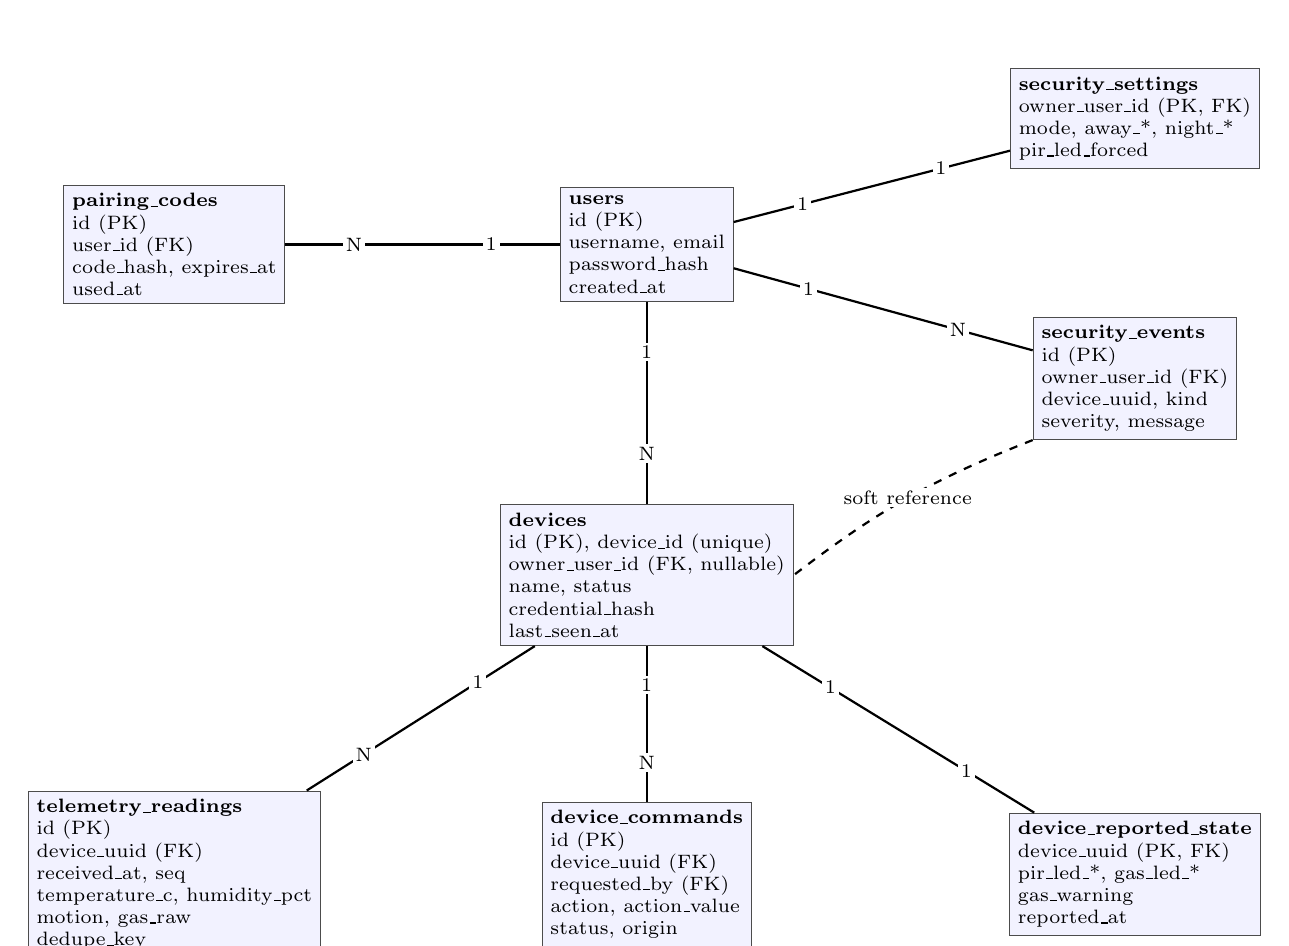
\begin{tikzpicture}[x=1cm,y=1cm]
  \node[entity] (users) at (0,0) {\textbf{users}\\id (PK)\\username, email\\password\_hash\\created\_at};
  \node[entity] (pc) at (-6,0) {\textbf{pairing\_codes}\\id (PK)\\user\_id (FK)\\code\_hash, expires\_at\\used\_at};
  \node[entity] (ss) at (6.2,1.6) {\textbf{security\_settings}\\owner\_user\_id (PK, FK)\\mode, away\_*, night\_*\\pir\_led\_forced};
  \node[entity] (se) at (6.2,-1.7) {\textbf{security\_events}\\id (PK)\\owner\_user\_id (FK)\\device\_uuid, kind\\severity, message};
  \node[entity] (dev) at (0,-4.2) {\textbf{devices}\\id (PK), device\_id (unique)\\owner\_user\_id (FK, nullable)\\name, status\\credential\_hash\\last\_seen\_at};
  \node[entity] (tel) at (-6,-8) {\textbf{telemetry\_readings}\\id (PK)\\device\_uuid (FK)\\received\_at, seq\\temperature\_c, humidity\_pct\\motion, gas\_raw\\dedupe\_key};
  \node[entity] (cmd) at (0,-8) {\textbf{device\_commands}\\id (PK)\\device\_uuid (FK)\\requested\_by (FK)\\action, action\_value\\status, origin};
  \node[entity] (rs) at (6.2,-8) {\textbf{device\_reported\_state}\\device\_uuid (PK, FK)\\pir\_led\_*, gas\_led\_*\\gas\_warning\\reported\_at};
  \draw[thick] (users) -- node[lbl, near start]{1} node[lbl, near end]{N} (pc);
  \draw[thick] (users) -- node[lbl, near start]{1} node[lbl, near end]{N} (dev);
  \draw[thick] (users) -- node[lbl, near start]{1} node[lbl, near end]{1} (ss);
  \draw[thick] (users) -- node[lbl, near start]{1} node[lbl, near end]{N} (se);
  \draw[thick] (dev) -- node[lbl, near start]{1} node[lbl, near end]{N} (tel);
  \draw[thick] (dev) -- node[lbl, near start]{1} node[lbl, near end]{N} (cmd);
  \draw[thick] (dev) -- node[lbl, near start]{1} node[lbl, near end]{1} (rs);
  \draw[thick, dashed] (se.south west) to[bend right=8] node[lbl, pos=0.5]{soft reference} (dev.east);
\end{tikzpicture}}
\caption{Entity--relationship diagram: users, devices, telemetry, commands and security.}
\label{fig:er-core}
\end{figure}

\begin{figure}[H]
\centering
\resizebox{\textwidth}{!}{%
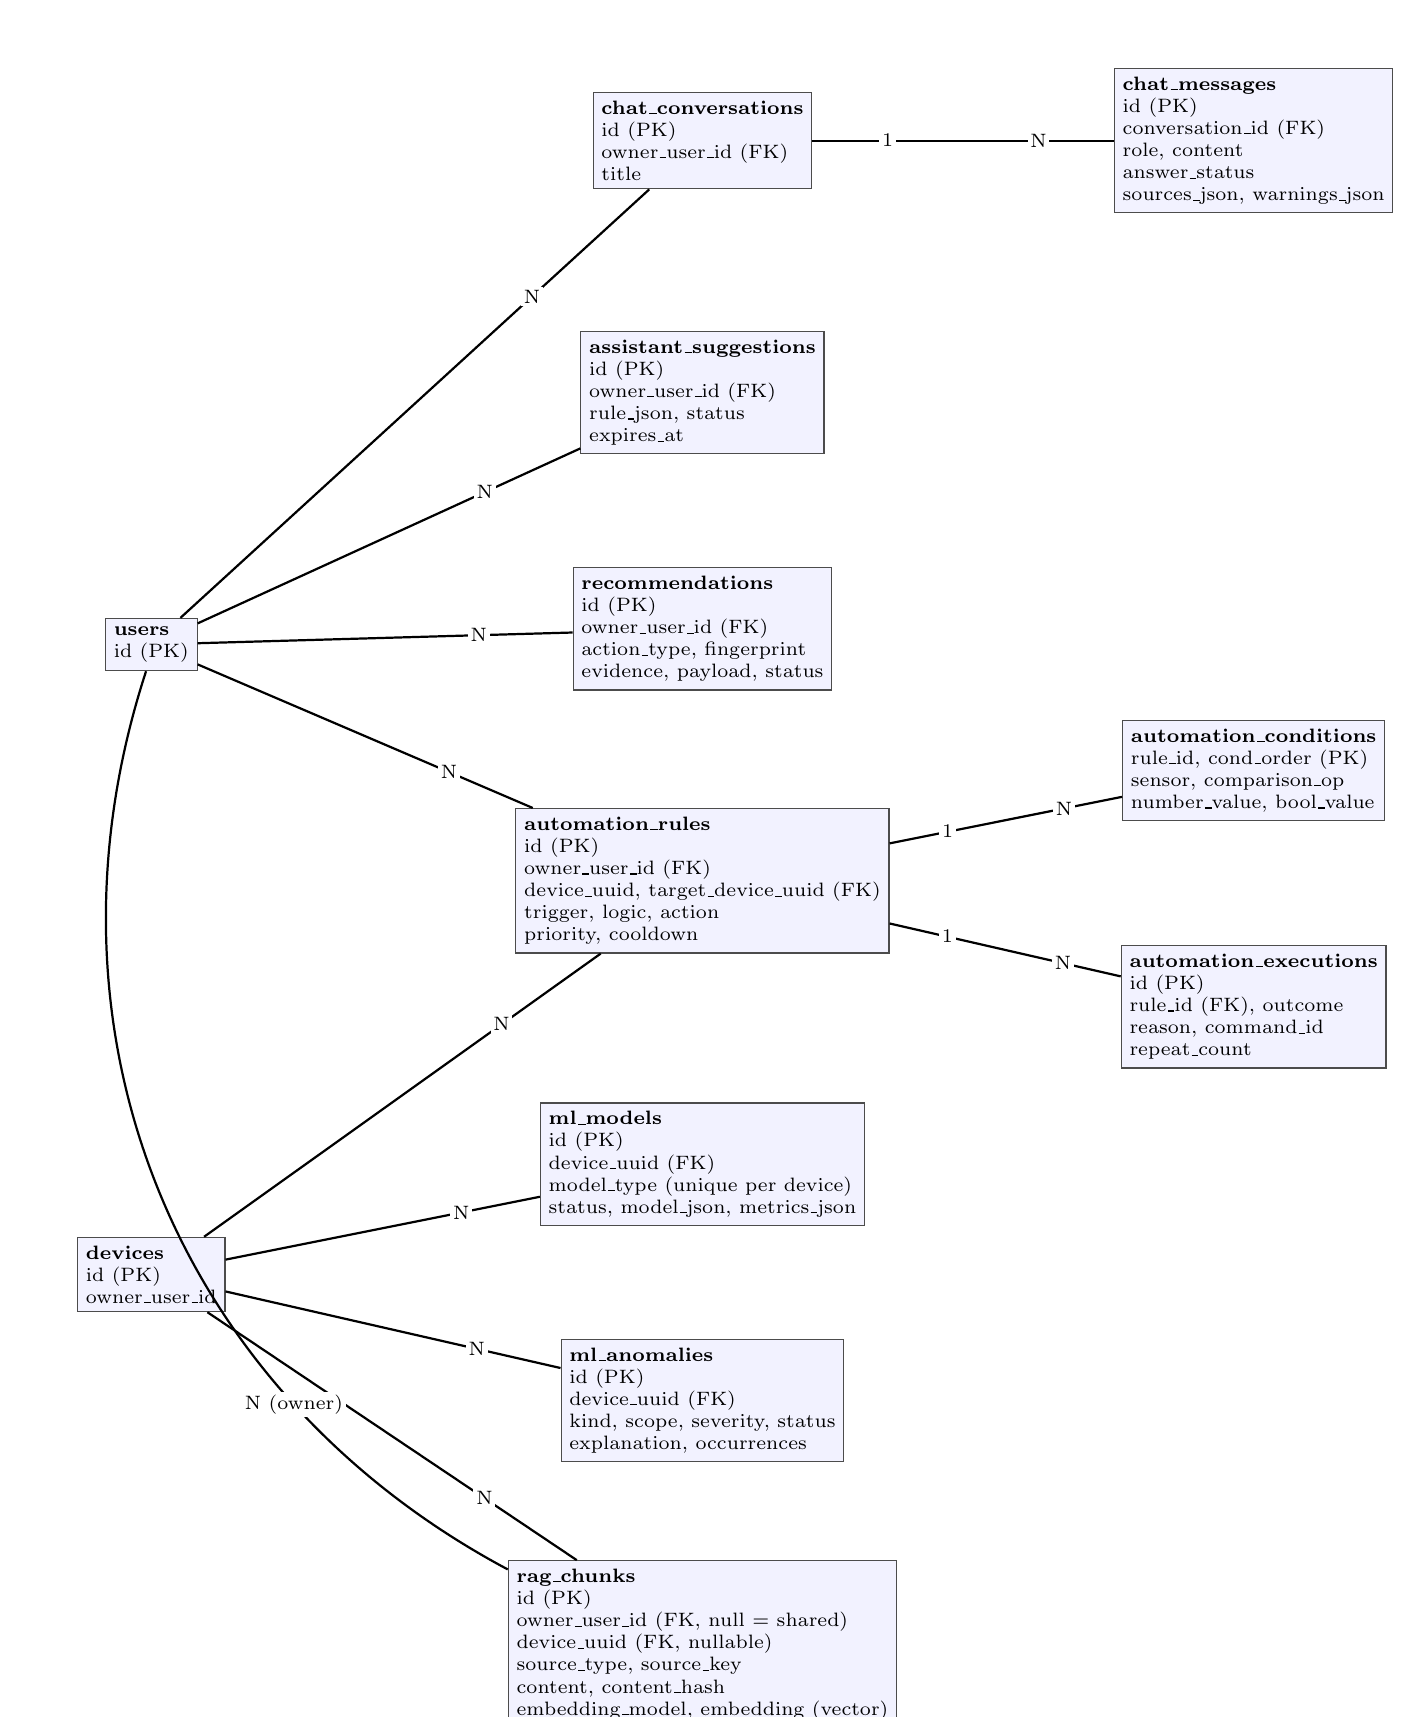
\begin{tikzpicture}[x=1cm,y=1cm]
  \node[entity] (users) at (0,0) {\textbf{users}\\id (PK)};
  \node[entity] (dev) at (0,-8) {\textbf{devices}\\id (PK)\\owner\_user\_id};
  \node[entity] (cc) at (7,6.4) {\textbf{chat\_conversations}\\id (PK)\\owner\_user\_id (FK)\\title};
  \node[entity] (cm) at (14,6.4) {\textbf{chat\_messages}\\id (PK)\\conversation\_id (FK)\\role, content\\answer\_status\\sources\_json, warnings\_json};
  \node[entity] (as) at (7,3.2) {\textbf{assistant\_suggestions}\\id (PK)\\owner\_user\_id (FK)\\rule\_json, status\\expires\_at};
  \node[entity] (rec) at (7,0.2) {\textbf{recommendations}\\id (PK)\\owner\_user\_id (FK)\\action\_type, fingerprint\\evidence, payload, status};
  \node[entity] (ar) at (7,-3) {\textbf{automation\_rules}\\id (PK)\\owner\_user\_id (FK)\\device\_uuid, target\_device\_uuid (FK)\\trigger, logic, action\\priority, cooldown};
  \node[entity] (ac) at (14,-1.6) {\textbf{automation\_conditions}\\rule\_id, cond\_order (PK)\\sensor, comparison\_op\\number\_value, bool\_value};
  \node[entity] (ae) at (14,-4.6) {\textbf{automation\_executions}\\id (PK)\\rule\_id (FK), outcome\\reason, command\_id\\repeat\_count};
  \node[entity] (ml) at (7,-6.6) {\textbf{ml\_models}\\id (PK)\\device\_uuid (FK)\\model\_type (unique per device)\\status, model\_json, metrics\_json};
  \node[entity] (an) at (7,-9.6) {\textbf{ml\_anomalies}\\id (PK)\\device\_uuid (FK)\\kind, scope, severity, status\\explanation, occurrences};
  \node[entity] (rag) at (7,-12.7) {\textbf{rag\_chunks}\\id (PK)\\owner\_user\_id (FK, null = shared)\\device\_uuid (FK, nullable)\\source\_type, source\_key\\content, content\_hash\\embedding\_model, embedding (vector)};
  \draw[thick] (users) -- node[lbl, near end]{N} (cc);
  \draw[thick] (cc) -- node[lbl, near start]{1} node[lbl, near end]{N} (cm);
  \draw[thick] (users) -- node[lbl, near end]{N} (as);
  \draw[thick] (users) -- node[lbl, near end]{N} (rec);
  \draw[thick] (users) -- node[lbl, near end]{N} (ar);
  \draw[thick] (ar) -- node[lbl, near start]{1} node[lbl, near end]{N} (ac);
  \draw[thick] (ar) -- node[lbl, near start]{1} node[lbl, near end]{N} (ae);
  \draw[thick] (dev) -- node[lbl, near end]{N} (ar);
  \draw[thick] (dev) -- node[lbl, near end]{N} (ml);
  \draw[thick] (dev) -- node[lbl, near end]{N} (an);
  \draw[thick] (dev) -- node[lbl, near end]{N} (rag);
  \draw[thick] (users) to[bend right=40] node[lbl, near end]{N (owner)} (rag);
\end{tikzpicture}}
\caption{Entity--relationship diagram: automation, machine learning, assistant and recommendations.}
\label{fig:er-intel}
\end{figure}

\section{Design Notes}
\begin{itemize}
  \item \textbf{Missing is not zero.} Sensor columns in \code{telemetry_readings} are nullable; a reading without a value stores null.
  \item \textbf{Secrets are hashed.} Pairing codes and device credentials are stored only as SHA-256 hashes; passwords as BCrypt hashes.
  \item \textbf{Vector column.} On PostgreSQL the column is an unconstrained \code{vector}; each row records its embedding model and dimension, and a search filters on both, so changing the embedding model never needs a schema change. Searches are exact; no approximate index is built because each user's corpus is small.
  \item \textbf{Portable tests.} Flyway's \texttt{\{vendor\}} location selects the pgvector script on PostgreSQL and a text-column script on H2, which the automated tests use.
\end{itemize}

% =====================================================================================
%  CHAPTER 9  API OVERVIEW
% =====================================================================================
\chapter{API Overview}
\label{ch:api}

Table~\ref{tab:api} summarises the endpoints. All endpoints return JSON. Errors have the form \texttt{\{status, error, message, fieldErrors?\}}. Unless marked otherwise, an endpoint requires a user JWT (\code{Authorization: Bearer ...}) and the user is taken from the token. Another user's resource always yields 404. The interface follows REST principles~\cite{fielding2000rest}: resources are addressed by URL and manipulated with standard HTTP methods.

\begin{longtable}{@{}p{1.8cm}p{6.2cm}p{6.3cm}@{}}
\caption{REST API summary}\label{tab:api}\\
\toprule
\textbf{Method} & \textbf{Path} & \textbf{Purpose}\\
\midrule
\endfirsthead
\toprule
\textbf{Method} & \textbf{Path} & \textbf{Purpose}\\
\midrule
\endhead
\multicolumn{3}{@{}l}{\textit{Public and authentication}}\\
GET & \api{/api/health} & Liveness check (no login).\\
POST & \api{/api/auth/register} & Create an account; returns a JWT.\\
POST & \api{/api/auth/login} & Log in; returns a JWT.\\
GET & \api{/api/auth/me} & Profile of the caller.\\
\midrule
\multicolumn{3}{@{}l}{\textit{Devices}}\\
POST & \api{/api/devices/pairing-codes} & Create a one-time pairing code.\\
GET & \api{/api/devices} & Own devices with connection state and latest reading.\\
GET & \api{/api/devices/{id}} & One device.\\
GET & \api{/api/devices/{id}/telemetry} & Recent readings, newest first (limit up to 200).\\
PATCH & \api{/api/devices/{id}} & Rename.\\
DELETE & \api{/api/devices/{id}} & Disown.\\
POST & \api{/api/device/pair} & Device side: claim with a pairing code (no login).\\
GET & \api{/api/device/me} & Device side: check own credential (device headers).\\
\midrule
\multicolumn{3}{@{}l}{\textit{Commands}}\\
POST & \api{/api/devices/{id}/commands} & Send an LED command (202; 400, 409, 429, 503 on problems).\\
GET & \api{/api/devices/{id}/commands} & Command history.\\
GET & \api{/api/devices/{id}/commands/{commandId}} & One command (poll its status).\\
\midrule
\multicolumn{3}{@{}l}{\textit{Automation}}\\
POST, GET & \api{/api/automations} & Create / list rules.\\
GET, PUT, DELETE & \api{/api/automations/{id}} & Read / replace / delete a rule.\\
PATCH & \api{/api/automations/{id}/enabled} & Enable or disable.\\
GET & \api{/api/automations/{id}/executions} & Audit trail of one rule.\\
GET & \api{/api/automations/executions} & Audit trail of all rules.\\
\midrule
\multicolumn{3}{@{}l}{\textit{Machine learning (per device)}}\\
GET & \api{/api/devices/{id}/ml/status} & Readiness, counts, metrics, anomaly summary.\\
POST & \api{/api/devices/{id}/ml/occupancy/train} & Train now (429 if repeated within 30\,s; 409 if running).\\
GET & \api{/api/devices/{id}/ml/occupancy/predict} & One prediction (409 without a usable model).\\
GET & \api{/api/devices/{id}/ml/occupancy/forecast} & Forecast points.\\
GET & \api{/api/devices/{id}/ml/anomalies} & Anomaly history (active or all).\\
PATCH & \api{/api/devices/{id}/ml/anomalies/{anomalyId}} & Acknowledge, resolve or dismiss.\\
POST & \api{/api/devices/{id}/ml/anomalies/scan} & Check now.\\
\midrule
\multicolumn{3}{@{}l}{\textit{Assistant}}\\
GET & \api{/api/assistant/status} & Model and embedding configuration (never a key), index size, limits.\\
POST & \api{/api/assistant/chat} & Ask a question; returns answer, status, sources, warnings, suggestions.\\
GET, DELETE & \api{/api/assistant/conversations...} & List conversations, read messages, delete.\\
GET, POST, DELETE & \api{/api/assistant/documents...} & User notes.\\
GET & \api{/api/assistant/suggestions} & Pending rule suggestions.\\
POST & \api{/api/assistant/suggestions/{id}/approve} & Approve: the only way a suggestion becomes a rule.\\
POST & \api{/api/assistant/suggestions/{id}/reject} & Reject.\\
\midrule
\multicolumn{3}{@{}l}{\textit{Security, twin, recommendations, status}}\\
GET & \api{/api/security/settings} & Mode, Away/Night settings, unacknowledged alerts.\\
PUT & \api{/api/security/mode} & Change mode.\\
PUT & \api{/api/security/config} & Change Away/Night behaviour.\\
GET & \api{/api/security/events} & Event history (filter by kind, limit).\\
POST & \api{/api/security/events/{id}/acknowledge} & Acknowledge one event.\\
POST & \api{/api/security/events/acknowledge-all} & Acknowledge all alerts.\\
GET & \api{/api/twins} & Digital twins of all own devices.\\
GET & \api{/api/devices/{id}/twin} & One twin.\\
GET & \api{/api/recommendations} & Pending recommendations with notes.\\
POST & \api{/api/recommendations/refresh} & Regenerate (rate limited).\\
POST & \api{/api/recommendations/{id}/approve} & Apply a recommendation.\\
POST & \api{/api/recommendations/{id}/dismiss} & Dismiss.\\
GET & \api{/api/system/status} & Authenticated system status.\\
\bottomrule
\end{longtable}

% =====================================================================================
%  CHAPTER 10  ALGORITHMS
% =====================================================================================
\chapter{Algorithms}
\label{ch:algorithms}

\section{Presence and De-duplication}
A device $d$ is \textsc{Online} at time $t$ exactly when
\begin{equation}
  \text{reported}(d)=\text{online}\ \wedge\ t-\text{lastSeen}(d)\le\tau,\qquad \tau=90\ \text{s (default)}.
\end{equation}
Redelivered MQTT messages are removed by a key $k=\mathrm{SHA\text{-}256}(\text{payload})$: a message whose key was already stored for the same device within ten minutes is dropped.

\section{Occupancy Model}
\subsection{Training examples}
Time is divided into 15-minute slots. A slot with at least 10 motion readings becomes an example; its label is $y=1$ if any reading in the slot reported motion and $y=0$ otherwise. Slots with fewer readings are dropped (they are \emph{not} labelled empty).

\subsection{Features}
Let $\theta\in[0,1)$ be the local time of day as a fraction of 24 hours (the time zone is chosen at training). The feature vector $\mathbf{x}\in\mathbb{R}^{30}$ consists of
\begin{itemize}
  \item the 12 harmonic terms $\sin(2\pi k\theta),\ \cos(2\pi k\theta)$ for $k=1,\dots,6$;
  \item 6 weekday indicators (Monday is the baseline);
  \item 12 weekend$\times$harmonic interaction terms, so that weekend and weekday daily shapes can differ.
\end{itemize}
Six harmonics were needed: a test with three harmonics smoothed a two-hour morning peak too much (predicted 0.52 against a true 0.85), so the number was raised to six.

\subsection{Model and fitting}
The model is logistic regression,
\begin{equation}
  P(y=1\mid\mathbf{x})=\sigma(b+\mathbf{w}^{\top}\mathbf{x}),\qquad \sigma(z)=\frac{1}{1+e^{-z}} ,
\end{equation}
fitted by minimising the ridge-penalised negative log-likelihood (the intercept $b$ is not penalised)~\cite{hastie2009esl}:
\begin{equation}
  J(\boldsymbol\beta)=-\sum_{i=1}^{n}\Big[y_i\ln p_i+(1-y_i)\ln(1-p_i)\Big]+\frac{\lambda}{2}\lVert\mathbf{w}\rVert_2^2 ,\qquad \lambda=1 .
\end{equation}
With $\boldsymbol\beta=(b,\mathbf{w})$, design matrix $X$ (with a column of ones), $S=\mathrm{diag}\big(p_i(1-p_i)\big)$ and penalty matrix $P$ (zero for the intercept), the Newton step, which is the same as iteratively reweighted least squares, is
\begin{equation}
  \boldsymbol\beta\leftarrow\boldsymbol\beta-H^{-1}\mathbf{g},\qquad
  \mathbf{g}=X^{\top}(\mathbf{p}-\mathbf{y})+\lambda P\boldsymbol\beta,\qquad
  H=X^{\top}SX+\lambda P .
\end{equation}
A backtracking line search keeps $J$ decreasing, and the procedure is deterministic.

\begin{algorithm}[H]
\caption{Occupancy training run}
\label{alg:train}
\begin{algorithmic}[1]
\State load motion readings of the last 28 days (capped), bucket them into 15-minute slots, drop slots with fewer than 10 readings
\If{usable slots, distinct days or examples of either class are below the minimum}
  \State store status \textsc{InsufficientData} with the reason; keep any earlier working model; \textbf{stop}
\EndIf
\State split the slots \emph{chronologically}: earliest 80\% for fitting, latest 20\% for testing
\State fit the evaluation model on the fitting part (Newton/IRLS with ridge)
\State compute metrics on the test part and the baseline (always predict the training rate)
\State \textbf{if} the model does not beat the baseline or $\mathrm{AUC}<0.6$ \textbf{then} status $\leftarrow$ \textsc{LowQuality} \textbf{else} \textsc{Ready}
\State refit on all slots and store the model, its metrics and per-hour-of-week support counts
\end{algorithmic}
\end{algorithm}

\subsection{Evaluation metrics}
With $n$ test slots and predictions $\hat p_i$, thresholded at 0.5:
\begin{align}
  \text{accuracy}&=\frac{TP+TN}{n}, &
  \text{precision}&=\frac{TP}{TP+FP}, &
  \text{recall}&=\frac{TP}{TP+FN},\\
  \text{log loss}&=-\frac1n\sum_i\big[y_i\ln\hat p_i+(1-y_i)\ln(1-\hat p_i)\big], &
  \text{Brier}&=\frac1n\sum_i(\hat p_i-y_i)^2 .
\end{align}
The area under the ROC curve is computed from ranks (Mann--Whitney form)~\cite{fawcett2006roc}; the Brier score is the mean squared error of probability forecasts~\cite{brier1950}. A measure that is undefined for the data (for example precision with no predicted positives, or AUC with one class) is returned as \emph{null}, never as zero. The baseline predicts the training positive rate $\bar p$ for every slot, and its accuracy and log loss are reported next to the model's.

\subsection{Prediction and confidence}
For a time $t$ the model gives $\hat p$. The \emph{confidence} is $\max(\hat p,1-\hat p)$. The \emph{support} is the number of training slots with the same weekday and hour; a prediction with support below 4, or from a \textsc{LowQuality} model, is marked unreliable.

\section{Anomaly Detection}
\subsection{Robust z-score}
For a sensor, let $B$ be the device's own baseline values (last 7 days excluding the last 30 minutes; the same hour of day $\pm1$ hour when at least 30 values exist, otherwise all hours; no judgement if fewer than 200 values). With $m=\mathrm{median}(B)$ and the median absolute deviation $\mathrm{MAD}=\mathrm{median}\,|b-m|$, a new value $x$ has the robust score
\begin{equation}
  z=\frac{x-m}{1.4826\cdot\max(\mathrm{MAD},\ s_{\min})} ,
\end{equation}
where the factor 1.4826 makes the MAD consistent with the standard deviation for normally distributed data, and $s_{\min}$ is a per-sensor floor that prevents a near-constant history from producing huge scores. The median and MAD are used instead of the mean and standard deviation because a few extreme values barely move them~\cite{leys2013mad}. The severity is WARNING for $|z|\ge4$ and CRITICAL for $|z|\ge6$. The stored explanation quotes the value, the median, the score and the number of baseline samples.

\subsection{Other detectors}
Plausibility limits, repeated values, missing values and silence are deterministic rules (Table~\ref{tab:anomaly-kinds}). Outcomes are de-duplicated: one row per ongoing problem, with an occurrence counter; conditions that end are closed automatically as \code{AUTO_RESOLVED}.

\begin{algorithm}[H]
\caption{Anomaly scan of one device}
\label{alg:scan}
\begin{algorithmic}[1]
\State read recent readings since the last watermark; build (or reuse a cached) baseline per sensor
\For{each reading and sensor}
  \State \textbf{if} value is absent \textbf{then} update the missing-data counter; \textbf{continue}
  \State check plausibility range; update the repeated-value counter
  \If{baseline has $\ge200$ samples} \State compute $z$; raise WARNING/CRITICAL if the threshold is exceeded \EndIf
\EndFor
\State check the time since the last message for staleness
\State create or update one row per ongoing problem; auto-resolve problems that have ended
\end{algorithmic}
\end{algorithm}

\section{Retrieval}
\subsection{Hashing embedder}
For a text, features are the word stems (stop words, long identifiers and UUIDs removed), a synonym token for a small table of smart-home words, and adjacent-word pairs. If feature $f$ occurs $c_f$ times with base weight $a_f$ (1.0 for words, 0.8 for synonyms, 0.5 for pairs), it contributes $a_f\,(1+\ln c_f)$ to coordinate $h(f)\bmod 256$ with sign given by the top bit of the 64-bit FNV-1a hash $h(f)$ (feature hashing~\cite{weinberger2009hash}). The vector is then normalised to unit length. Cosine similarity of two such vectors measures shared vocabulary.

\subsection{Similarity search}
With unit vectors $\mathbf{u},\mathbf{v}$, the similarity is $\cos(\mathbf{u},\mathbf{v})=\mathbf{u}\cdot\mathbf{v}$. In pgvector the cosine distance operator returns $1-\cos$, so the reported score is
\begin{equation}
  s(\mathbf{q},\mathbf{c})=1-d_{\cos}(\mathbf{q},\mathbf{c}),
\end{equation}
and chunks scoring below a minimum (0.12 by default for the built-in embedder) are not evidence. The query is restricted by \texttt{owner = caller OR owner IS NULL}.

\subsection{Re-ranking}
A wider candidate pool ($4K$ chunks) is re-ranked with a small boost for chunks about a device whose name appears in the question:
\begin{equation}
  s'=s+\beta,\qquad \beta=\begin{cases}0.20&\text{status chunk of a named device}\\0.15&\text{other chunk of a named device}\\0&\text{otherwise,}\end{cases}
\end{equation}
and the top $K=6$ are kept. The boost only reorders chunks that the owner-scoped search already returned.

\subsection{Grounding check}
Let $N_a$ be the numbers appearing in the answer and $N_s$ those in the retrieved sources and the question. A number $x$ written with $d$ decimals is accepted if some $y\in N_s$ satisfies $\mathrm{round}_d(|y|)=|x|$ (so rounding to fewer decimals is allowed). Whole numbers from 0 to 10 without a unit are exempt. Timestamps contribute only their whole-number parts, so fractional seconds cannot confirm an invented reading. Numbers that cannot be matched are reported to the user.

\begin{algorithm}[H]
\caption{Answering a question}
\label{alg:answer}
\begin{algorithmic}[1]
\State validate the message; apply the per-user rate limit (15 per minute)
\State refresh the user's live facts (hash-skipped); embed the question
\State retrieve the top candidates for this user; re-rank; keep $K$
\If{nothing is retrieved} \State return \textsc{NoContext} (the model is not called) \EndIf
\If{no model is configured} \State return \textsc{NotConfigured} with the retrieved records \EndIf
\State build the prompt (fixed rules; fenced, neutralised context; question); call the model
\If{the call fails} \State return \textsc{LlmUnavailable} with the records and a safe reason \EndIf
\State split off an optional rule proposal; run the grounding check on the visible text
\State validate the proposal with the rule validator and ownership checks; store it as \textsc{Pending} or discard it with a warning
\State store and return the answer, sources, warnings and proposal
\end{algorithmic}
\end{algorithm}

\section{Recommendations}
\paragraph{Quiet hours.} From the 24-hour forecast let $q_h=1$ if the hour $h$ is backed by enough similar slots and $\hat p_h<0.10$. The longest cyclic run of consecutive hours with $q_h=1$ is selected; if its length is at least four, two schedule rules are proposed (start: PIR LED off; end: PIR LED auto).
\paragraph{Temperature indicator.} If at least three unusual temperature readings occurred in 7 days and at least 200 temperature values exist, the threshold is
\begin{equation}
  \vartheta=\tfrac12\,\mathrm{round}\big(2\,(P_{95}+2)\big)\ \ {}^{\circ}\mathrm{C},
\end{equation}
where $P_{95}$ is the 95th percentile of the stored temperatures; a proposal is only made if $\vartheta<80$.
\paragraph{Failing rules.} For an enabled rule with at least 5 runs in 7 days, if the share of failed or target-offline runs is at least 0.7, disabling is proposed.

\section{Digital Twin Decision}
For one output the state is chosen in this order: \textsc{Pending} if a command is in flight; else \textsc{NoDesired} if no command was acknowledged; else \textsc{Unreported} if the state report is missing or stale; else \textsc{Unknown} if an unacknowledged later command exists; else \textsc{InSync} if the reported mode equals the last acknowledged value, otherwise \textsc{Drift}.

\section{Back-off and Rate Limits}
Reconnection delays on the device grow as $\min\big(D_{\max},D_{\min}2^{n}\big)$ with 20\% random jitter, with $(D_{\min},D_{\max})=(1,60)$\,s for Wi-Fi and $(2,120)$\,s for MQTT. Server-side limits use sliding windows or minimum intervals: chat 15 messages per minute per user, manual training once per 30 seconds per device, anomaly checks and recommendation refresh with short minimum intervals, and at most five commands waiting per device.

% =====================================================================================
%  CHAPTER 11  SECURITY
% =====================================================================================
\chapter{Security Analysis}
\label{ch:security}

\section{Threats and Controls}
Table~\ref{tab:threats} lists the main threats considered, the controls implemented in the code, and where each is exercised by tests. ``Live'' means it was also exercised against the real PostgreSQL and Mosquitto instances.

\begin{longtable}{@{}p{3.0cm}p{6.2cm}p{5.4cm}@{}}
\caption{Threat and control summary}\label{tab:threats}\\
\toprule
\textbf{Threat} & \textbf{Control} & \textbf{Verification}\\
\midrule
\endfirsthead
\toprule
\textbf{Threat} & \textbf{Control} & \textbf{Verification}\\
\midrule
\endhead
Stolen password database & BCrypt hashes; passwords limited to 72 bytes; no password ever logged. & Auth tests.\\
Forged or expired tokens & HS256 signature, expiry and issuer checked on each request; secret of at least 32 characters required from the environment; stateless API. & Auth tests.\\
Reading or changing another user's data & Owner taken from the JWT; every query includes the owner; foreign resources reported as ``not found''; assistant retrieval filtered by owner in SQL and checked again in code. & Ownership tests in every module (devices, commands, rules, ML, assistant, security, twin, recommendations, status); live checks.\\
Claiming someone else's device & One-time pairing code, 10-minute lifetime, hashed, rate limited per client; the hardware ID or MAC alone is never proof. & Device tests.\\
Rogue MQTT client & Anonymous access off; per-device accounts confined to their own topics; only the backend may publish commands. & Live broker checks documented in the README: wildcard and other-device subscriptions refused, forged commands and acknowledgements never delivered.\\
Command replay, delay or misdelivery & UUID, absolute expiry, QoS~1 not retained, device-side validation, idempotence on the device, guarded status transitions, acknowledgement. & Command tests; live.\\
Suppressing the gas warning & No ``off'' for the gas LED in the allow-list; refused again in the API, the command service, the automation engine (three layers) and the firmware; security modes, recommendations and the assistant can only build PIR-LED actions or have proposals validated by the same rules. & Automation, command, security, recommendation and assistant tests; live (no gas-LED command ever created).\\
Malformed or flooding telemetry & Size, range and timestamp limits; de-duplication; bounded queues; invalid messages logged by reason only. & Telemetry tests.\\
SQL or code injection & Parameterised JPA/JDBC queries; rules are data with a fixed vocabulary (no expressions). & Validator and rule tests.\\
Prompt injection through stored text & Stored text is fenced as data, neutralised, never in the system message; the model has no tool to act; proposals are validated and need approval. & Prompt-builder tests; chat tests with a model that obeys the injection.\\
Invented facts from the assistant & No model call without retrieved evidence; numbers checked against sources; sources always shown. & Grounding tests; chat tests.\\
Secret leakage & Secrets only in a git-ignored \code{.env} or the environment; keys only in request headers; generic client error messages; prompts contain no tokens or credentials. & Tests; live log scans found none of the configured secrets.\\
Cross-site scripting & React escapes text; assistant output is rendered as plain text. & Design (not browser-tested).\\
Eavesdropping on the LAN & Not addressed: MQTT and HTTP are unencrypted in this prototype. & Documented limitation.\\
Physical access to a board & Not addressed: the credential in flash is not encrypted by default. & Documented limitation.\\
\bottomrule
\end{longtable}

\section{Defence in Depth for the Gas Warning}
The gas warning is the one function whose failure could matter physically, so it is protected at every layer (Figure~\ref{fig:gas-layers}). The innermost layer is in the firmware and does not depend on any network or software above it.

\begin{figure}[H]
\centering
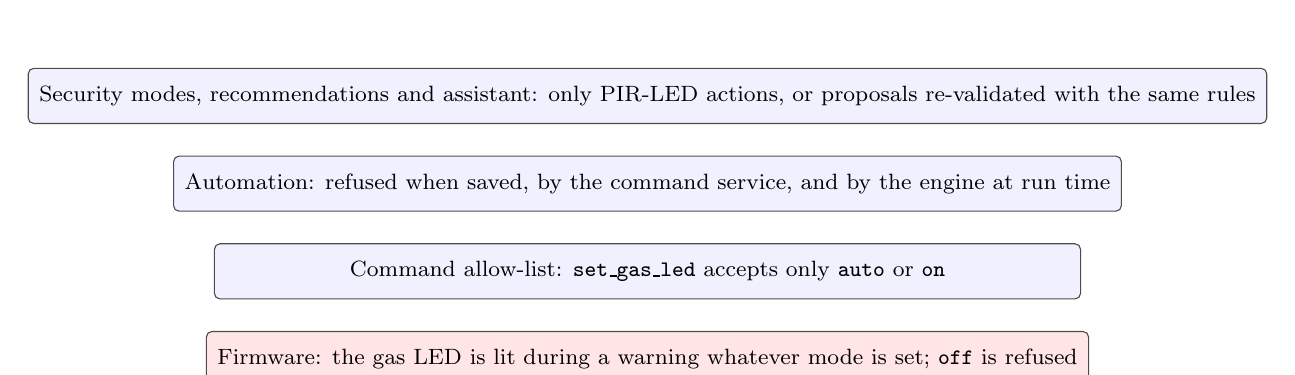
\begin{tikzpicture}[node distance=4mm]
  \node[box, minimum width=11cm, fill=red!10] (a) {Firmware: the gas LED is lit during a warning whatever mode is set; \texttt{off} is refused};
  \node[box, minimum width=11cm, above=of a] (b) {Command allow-list: \texttt{set\_gas\_led} accepts only \texttt{auto} or \texttt{on}};
  \node[box, minimum width=11cm, above=of b] (c) {Automation: refused when saved, by the command service, and by the engine at run time};
  \node[box, minimum width=11cm, above=of c] (d) {Security modes, recommendations and assistant: only PIR-LED actions, or proposals re-validated with the same rules};
\end{tikzpicture}
\caption{Layers protecting the gas warning (innermost at the bottom).}
\label{fig:gas-layers}
\end{figure}
None of these layers makes the system a certified gas-safety device; the README and the in-application notices say so explicitly.

% =====================================================================================
%  CHAPTER 12  INSTALLATION AND EXECUTION
% =====================================================================================
\chapter{Installation and Execution}
\label{ch:install}

\section{Prerequisites}
JDK 21 or newer, Node.js 20 or newer, and Docker Desktop (running). Maven is not required because the Maven wrapper is bundled. For the firmware: the Arduino CLI (or Arduino IDE~2) with the ESP32 core, which needs about 5~GB of disk space.

\section{Configuration}
Copy the template and edit the copy; never commit it. Choose real values for the database password, the JWT secret (at least 32 characters) and the two broker passwords.

\begin{lstlisting}[language={},caption={Preparing the environment file (PowerShell)}]
copy .env.example .env
# edit .env: POSTGRES_PASSWORD, JWT_SECRET, MQTT_ADMIN_PASSWORD, MQTT_BACKEND_PASSWORD
# a random secret can be generated with:
[Convert]::ToBase64String((1..48 | % { Get-Random -Max 256 }))
\end{lstlisting}

If a port is already in use, change \code{POSTGRES_PORT}, \code{MQTT_PORT} or \code{SERVER_PORT} in \code{.env}; if \code{SERVER_PORT} changes, start the frontend with \code{VITE_API_TARGET} pointing at it and add the frontend origin to \code{CORS_ALLOWED_ORIGINS}. Appendix~\ref{app:config} (Table~\ref{tab:env}) lists all variables (names only).

\section{Running the System}
\begin{lstlisting}[language={},caption={Start the database and broker, the backend and the frontend}]
# 1. database and broker
docker compose up -d
docker compose ps -a

# 2. backend (applies migrations, creates broker roles, connects to MQTT)
cd backend
.\mvnw.cmd spring-boot:run

# 3. frontend
cd frontend
npm install
npm run dev
\end{lstlisting}
Open the address that Vite prints (normally \code{http://localhost:5173}), register, and use the Devices page.

\section{Enabling the Assistant's Language Model (Optional)}
Without any \code{LLM_*} variable the assistant still searches the user's data and shows the matching records. To get written answers, set \code{LLM_PROVIDER} to \code{openai} (any OpenAI-compatible server, for example a local Ollama server) or \code{anthropic}, plus \code{LLM_MODEL} and, when needed, \code{LLM_BASE_URL} and \code{LLM_API_KEY} in \code{.env}, and restart the backend. For meaning-based search, set \code{EMBEDDING_PROVIDER} to \code{openai} and \code{EMBEDDING_MODEL}.

\section{Building and Flashing the Firmware}
\begin{lstlisting}[language={},caption={Firmware toolchain and build (Arduino CLI)}]
arduino-cli config init
arduino-cli config add board_manager.additional_urls https://espressif.github.io/arduino-esp32/package_esp32_index.json
arduino-cli core update-index
arduino-cli core install esp32:esp32
arduino-cli lib install "DHT sensor library" "Adafruit Unified Sensor" "PubSubClient" "ArduinoJson"

cd firmware\smarthome_esp32s3
copy secrets.example.h secrets.h      # then enter Wi-Fi and the PC's LAN address

cd ..\..
arduino-cli compile --fqbn esp32:esp32:esp32s3 firmware\smarthome_esp32s3
arduino-cli upload  --fqbn esp32:esp32:esp32s3 -p COM5 firmware\smarthome_esp32s3
arduino-cli monitor -p COM5 -c baudrate=115200
\end{lstlisting}
The API and broker addresses in \code{secrets.h} must be the PC's LAN address (not \code{localhost}); Windows Firewall must allow inbound connections on both ports. Pair the board by creating a code in the web application and typing it into the Serial Monitor.

\section{Running the Tests}
\begin{lstlisting}[language={},caption={Automated checks}]
cd backend;  .\mvnw.cmd verify          # backend build and all automated tests
cd frontend; npm run build; npm run lint
\end{lstlisting}
The backend tests use an in-memory H2 database, a recording fake broker and a scripted fake language model, so they need no Docker and no API key.

% =====================================================================================
%  CHAPTER 13  TESTING AND RESULTS
% =====================================================================================
\chapter{Testing and Results}
\label{ch:testing}

\begin{center}
\fbox{\parbox{0.93\textwidth}{\small\textbf{What was and was not verified.} Every number in this chapter was produced by running the project's own tests or scripts during development. \textbf{Not done:} testing on a physical ESP32-S3 with real sensors; any call to a real large language model or real neural embedding model (the assistant was verified with a scripted fake and a local stub server that speaks the OpenAI chat format); manual testing of the web pages in a browser (they were compiled and linted only); performance or load testing; TLS. All machine-learning figures come from \emph{simulated} data created for testing and say nothing about the accuracy in a real home.}}
\end{center}

\section{Test Strategy}
\begin{itemize}
  \item \textbf{Unit tests} for pure logic: the condition evaluator, logistic regression, metrics, the occupancy trainer, anomaly detectors, the chunker, the embedder, the prompt builder, the grounding check, the suggestion parser, the re-ranker, the rate limiter and the HTTP model clients (against a local stub server).
  \item \textbf{Integration tests} start the whole Spring application with an in-memory database and drive it through real HTTP-level calls (MockMvc), including ownership, validation and failure cases. Telemetry, acknowledgements and state reports are fed through the same ingest code the MQTT client uses.
  \item \textbf{Live integration checks} start the backend against the real PostgreSQL (with pgvector) and Mosquitto containers and exercise the flows with scripts that stand in for devices, publishing over real MQTT with each device's own credential.
  \item \textbf{Firmware logic tests} (\code{firmware/tests}) compile the pure firmware logic and the command parser on a PC. They were run during development; their counts are not repeated here because they were not re-run for this report.
  \item \textbf{Frontend checks:} the TypeScript compiler and oxlint.
\end{itemize}

\section{Backend Test Results}
The command \code{mvnw verify} ran \textbf{372 tests with 0 failures and 0 errors}. Table~\ref{tab:testcounts} gives the counts per test class and Table~\ref{tab:cumulative} the cumulative growth.

\begin{longtable}{@{}p{2.2cm}p{9.0cm}r@{}}
\caption{Automated backend tests by chunk (counts from the last full run)}\label{tab:testcounts}\\
\toprule
\textbf{Chunk} & \textbf{Test class} & \textbf{Tests}\\
\midrule
\endfirsthead
\toprule
\textbf{Chunk} & \textbf{Test class} & \textbf{Tests}\\
\midrule
\endhead
2 & AuthTests & 6\\
3 & DeviceTests & 17\\
4 & TelemetryTests & 21\\
4 & DynsecErrorToleranceTest & 5\\
1 & SmarthomeBackendApplicationTests & 1\\
5 & CommandTests & 28\\
6 & ConditionEvaluatorTest & 9\\
6 & AutomationApiTests & 15\\
6 & AutomationEngineTests & 23\\
6 & AutomationScheduleTests & 12\\
7 & LogisticRegressionTest & 8\\
7 & ModelMetricsTest & 6\\
7 & OccupancyTrainerTest & 15\\
7 & AnomalyDetectorsTest & 18\\
7 & MlApiTests & 13\\
7 & MlAnomalyTests & 19\\
8 & ChunkerTest & 7\\
8 & LocalHashEmbeddingTest & 6\\
8 & GroundingCheckTest & 10\\
8 & PromptBuilderTest & 8\\
8 & SuggestionParserTest & 7\\
8 & RerankTest & 3\\
8 & ChatRateLimiterTest & 2\\
8 & HttpModelClientsTest & 12\\
8 & AssistantRagTests & 17\\
8 & AssistantChatTests & 26\\
9 & SecurityModeTests & 20\\
9 & DigitalTwinTests & 11\\
9 & RecommendationTests & 14\\
9 & SystemStatusTests & 13\\
\midrule
 & \textbf{Total} & \textbf{372}\\
\bottomrule
\end{longtable}

\subsection{Cumulative growth}
\begin{table}[H]
\centering
\caption{Cumulative automated tests after each stage}
\label{tab:cumulative}
\begin{tabular}{lrr}
\toprule
\textbf{After} & \textbf{New tests} & \textbf{Total}\\
\midrule
Chunks 1--6 & 137 & 137\\
Chunk 7 (ML) & 79 & 216\\
Chunk 8 (assistant) & 98 & 314\\
Chunk 9 (security, twin, recommendations, status) & 58 & 372\\
\bottomrule
\end{tabular}
\end{table}

\subsection{Examples of what the tests assert}
\begin{itemize}
  \item \textbf{Permissions:} every endpoint of every module returns 401 without a login; another user's device, rule, anomaly, conversation, suggestion, recommendation, security event or twin returns 404 and nothing changes.
  \item \textbf{Validation:} unknown modes, out-of-range cooldowns, oversized messages and notes, malformed JSON and invalid rules return 400 with field messages.
  \item \textbf{Gas protection:} an automation rule or an assistant proposal that switches the gas LED off is refused or discarded; running every security mode with a very high raw gas value creates no \code{set_gas_led} command.
  \item \textbf{Failure cases:} broker down (commands 503, status DOWN), model timeout, rejected key or crash (answer degrades to references), embedding service down (clear message, nothing guessed), database outage during chat (HTTP 503 without internal detail, recovers afterwards), device offline (command refused), missing sensor value (never zero).
  \item \textbf{Prompt injection:} a device name containing delimiter text cannot close the context block; a note instructing the model to create an unsafe rule is handed to a scripted model that obeys it, and the resulting proposal is still discarded.
  \item \textbf{Hallucination:} an invented temperature in a model reply is reported as unverified; a citation to a non-existent source is removed; with nothing retrieved the model is not called.
  \item \textbf{Concurrency and idempotence:} a second approval of a suggestion or recommendation returns 409 and creates no second rule; repeated motion inside the cooldown yields one alert.
\end{itemize}

\subsection{Defects found and fixed during testing}
Testing found real defects, which were fixed before the chunk was accepted: (i) work started from an after-commit callback silently lost its database writes, fixed by handing it to a dedicated worker thread; (ii) readings with identical timestamps made ``newest reading'' ambiguous, fixed with an identifier tie-break; (iii) three sine/cosine harmonics were too few for a sharp daily peak, so six are used; (iv) random identifiers changed the ranking of word-based embeddings and made tests intermittent, fixed by ignoring identifiers in the embedder; (v) fractional seconds of a timestamp could ``confirm'' an invented reading in the grounding check, fixed by using only the whole-number parts of timestamps; (vi) a regular-expression escape in a test produced a backspace character instead of a word boundary.

\section{Live Integration Results}
Table~\ref{tab:live} lists what was executed against the real PostgreSQL 17 (pgvector) and Mosquitto containers. Rows labelled \emph{simulated} used history inserted by the test script (marked in the database and deleted afterwards); the ``devices'' were scripts using the pairing flow and each device's own credential, not boards.

\begin{longtable}{@{}p{2.3cm}p{12.3cm}@{}}
\caption{Live integration checks}\label{tab:live}\\
\toprule
\textbf{Chunk} & \textbf{Observed result}\\
\midrule
\endfirsthead
\toprule
\textbf{Chunk} & \textbf{Observed result}\\
\midrule
\endhead
6 & Migration applied and schema validated; a telemetry rule, its cooldown, the ``no data'' skip, a scheduled rule and disown cleanup were exercised end to end over real MQTT.\\
7 & Migration V6 applied. With no data the model reported \code{INSUFFICIENT_DATA} with no metrics. With 14 days of \emph{simulated} one-reading-per-minute history (20\,160 rows) training reached \code{READY}; hold-out accuracy was 1.000 against a baseline of 0.743, log loss 0.037 against 0.574, on 269 test slots of which 69 had motion \simulated. These near-perfect values arise because the simulated pattern is easy and are \emph{not} an accuracy claim. Injected outlier, saturated-gas and frozen-gas readings were detected (temperature 48\,\degC\ scored 92.7 robust deviations above the simulated baseline); acknowledge, resolve, repeated-resolve (409) and invalid-status (400) behaved as designed; disowning removed all telemetry, models and anomalies. Immediate repeated training returned 429.\\
8 & Migrations V7 and V8 applied. 21 shared help chunks and the owner's chunks were stored as 256-dimension \code{vector} values; a native cosine-distance query returned a chunk's own text with score 1.000. With a local stub server standing in for the language model (\emph{not a real model}): the owner got a cited answer using the stored 23.4\,\degC; a second user's question about the first user's device sent nothing about it to the model; a suggested rule created nothing until approved (second approval 409, other user 404); a proposal to switch the gas LED off was discarded; a note was found by its owner only; model HTTP 500 and 401 degraded to references with a plain reason; disowning removed all eight chunks of the device.\\
9 & Migration V9 applied. Over real MQTT: the status view showed database and broker OK, the device online and all four sensors fresh; in Away mode one motion message produced one alert and a second inside the cooldown none; with the LED option the device received \code{set_pir_led on} on its command topic (origin \code{security:away}); the twin passed from pending to in sync after the acknowledgement and state report, then to drift when the device reported \emph{auto}; leaving Away delivered \code{set_pir_led auto}; no gas-LED command ever existed; another user received 404 on the twin and on acknowledging the alert. With \emph{simulated} 21-day motion history and a model trained on it (hold-out accuracy 0.99 against a baseline of 0.645 \simulated), the quiet-hours recommendations for 23:00 to 06:00 (highest motion chance 6.3\%) appeared; approving one created the rule, a second approval returned 409, a dismissed one was not offered again, and the refresh throttle returned 429. Stopping the Mosquitto container turned the status DOWN (``not connected'') and it returned to OK after the container restarted.\\
Logs & For the Chunk 7, 8 and 9 runs, the backend log contained none of the configured database, JWT, broker or language-model secrets, and no application error lines.\\
\bottomrule
\end{longtable}

\section{Frontend Results}
\code{npm run build} (TypeScript compilation followed by the Vite production build) passes after every chunk. \code{npm run lint} reports one cosmetic warning in the authentication context file (a fast-refresh recommendation); no other findings.

\section{Limits of the Evidence}
\begin{itemize}
  \item The firmware has \textbf{not} been executed on a physical ESP32-S3, so sensor accuracy, the calibration of the gas thresholds, Wi-Fi behaviour, power behaviour and the LED behaviour on real hardware are unverified.
  \item The assistant has \textbf{not} been validated with a real large language model. Answer quality, instruction following and the rate of unsupported statements with a real model are unknown. Retrieval quality was checked only with the built-in word-based embedder.
  \item The occupancy and anomaly figures come from simulated data. Performance on real homes, with real sensor noise and real behaviour, has not been measured.
  \item The web pages have been built and linted but not exercised by a person or by browser-automation tests in this project.
\end{itemize}

% =====================================================================================
%  CHAPTER 14  LIMITATIONS
% =====================================================================================
\chapter{Limitations}
\label{ch:limits}

\section{Hardware and Firmware}
\begin{itemize}
  \item No physical testing yet (Chapter~\ref{ch:testing}); the gas thresholds are placeholders that must be calibrated; the firmware's LED and gas behaviour was written from scratch.
  \item MQTT and HTTP are unencrypted; the device credential is stored unencrypted in flash.
  \item A hardware identifier is not a secret: after a device is disowned, anyone holding a valid pairing code could register that identifier (the genuine device would not have the new credential). Proving possession of the physical device would need a per-device secret installed at manufacture.
  \item Only two LEDs can be controlled; there are no relays or other actuators.
\end{itemize}

\section{Automation, Machine Learning and Security Modes}
\begin{itemize}
  \item Rules have one flat condition list with one AND/OR mode and read one device's sensors.
  \item ``Occupied'' means the PIR fired; a person sitting still may not trigger it. The model uses time features only; one time zone is fixed at training; anomaly baselines use UTC hours.
  \item Meaningful prediction needs about two weeks or more of real history.
  \item Security modes watch every device of the owner, have no automatic schedule, siren or phone notification, and the offline-while-armed memory is lost on a backend restart. It is not a certified alarm system.
  \item Sensor freshness uses one threshold for all sensors.
\end{itemize}

\section{Assistant}
\begin{itemize}
  \item A language model can still be wrong or incomplete; the checks catch only numbers missing from the sources and citations to nothing.
  \item The default embedder matches wording, not meaning; generic questions may miss the right records.
  \item Only the last seven days of readings are indexed, as daily summaries; live facts can be about ten seconds old; search is exact and suited to up to a few thousand chunks per user.
  \item Only OpenAI-compatible and Anthropic APIs are supported; no streaming and no tool calling.
\end{itemize}

\section{General}
The system is designed for a single home on a trusted network, not for multi-tenant internet deployment. Token storage in the browser's local storage is exposed to any script running on the page. No performance or load testing was done.

% =====================================================================================
%  CHAPTER 15  FUTURE SCOPE
% =====================================================================================
\chapter{Future Scope}
\label{ch:future}
\begin{enumerate}
  \item \textbf{Complete the hardware verification} (the fourteen-step checklist), calibrate the MQ-2 thresholds, and record real data for a period of weeks.
  \item \textbf{Evaluate the assistant with a real model} (hosted or local) and a neural embedding model; measure retrieval quality and the rate of unsupported answers on a set of real questions.
  \item \textbf{Transport security:} TLS for MQTT and the API, ESP32 flash encryption, and a per-device secret provisioned at manufacture.
  \item \textbf{More actuators and sensors:} relays and smart plugs, additional rooms, energy metering, and per-device security selection.
  \item \textbf{Richer intelligence:} features such as weather and holidays, per-device models for several rooms, user feedback on predictions and anomalies, and scheduled arming of Night mode.
  \item \textbf{Notifications:} push, e-mail or a local siren for security alerts.
  \item \textbf{Over-the-air firmware updates} with signed images.
  \item \textbf{Browser-level tests} for the user interface and accessibility review.
\end{enumerate}

% =====================================================================================
%  CHAPTER 16  CONCLUSION
% =====================================================================================
\chapter{Conclusion}
\label{ch:conclusion}
This project delivered a self-hosted smart-home platform whose backend, database, messaging, machine-learning, retrieval-augmented assistant and web application are implemented and verified by 372 passing automated tests and by integration checks against real PostgreSQL and Mosquitto instances. The main results are architectural as much as functional: a single modular monolith in which every action passes through one command path; ownership enforced once, in the services; a gas warning kept entirely on the microcontroller and protected at every software layer; machine-learning components that report insufficient data instead of guessing and compare themselves with a baseline; and an assistant that retrieves from the user's own records, shows its sources, checks its numbers and can only propose changes that a human approves.

The work also shows where care is needed. Testing found real defects, from lost writes in after-commit callbacks to random identifiers perturbing word-based embeddings, which would have been hard to find by inspection. Equally important are the limits stated in this report: the firmware has not been run on a physical board, the assistant has not been tried with a real language model, and the machine-learning figures come from simulated data. Closing those gaps is the natural next step (Chapter~\ref{ch:future}), and the architecture was built so that doing so requires configuration and measurement rather than redesign.

% =====================================================================================
%  REFERENCES
% =====================================================================================
\begin{thebibliography}{99}
\addcontentsline{toc}{chapter}{References}

\bibitem{mqtt311} A.~Banks and R.~Gupta (eds.), \emph{MQTT Version 3.1.1}, OASIS Standard, 29 October 2014.

\bibitem{rfc7519} M.~Jones, J.~Bradley and N.~Sakimura, ``JSON Web Token (JWT),'' RFC 7519, Internet Engineering Task Force, May 2015.

\bibitem{bcrypt} N.~Provos and D.~Mazi\`eres, ``A future-adaptable password scheme,'' in \emph{Proc. USENIX Annual Technical Conference, FREENIX Track}, 1999.

\bibitem{fielding2000rest} R.~T. Fielding, ``Architectural styles and the design of network-based software architectures,'' Ph.D. dissertation, University of California, Irvine, 2000.

\bibitem{lewis2020rag} P.~Lewis \emph{et al.}, ``Retrieval-augmented generation for knowledge-intensive NLP tasks,'' in \emph{Advances in Neural Information Processing Systems 33 (NeurIPS 2020)}, pp.~9459--9474, 2020.

\bibitem{hastie2009esl} T.~Hastie, R.~Tibshirani and J.~Friedman, \emph{The Elements of Statistical Learning}, 2nd ed., Springer, 2009.

\bibitem{fawcett2006roc} T.~Fawcett, ``An introduction to ROC analysis,'' \emph{Pattern Recognition Letters}, vol.~27, no.~8, pp.~861--874, 2006.

\bibitem{brier1950} G.~W. Brier, ``Verification of forecasts expressed in terms of probability,'' \emph{Monthly Weather Review}, vol.~78, no.~1, pp.~1--3, 1950.

\bibitem{leys2013mad} C.~Leys, C.~Ley, O.~Klein, P.~Bernard and L.~Licata, ``Detecting outliers: Do not use standard deviation around the mean, use absolute deviation around the median,'' \emph{Journal of Experimental Social Psychology}, vol.~49, no.~4, pp.~764--766, 2013.

\bibitem{weinberger2009hash} K.~Weinberger, A.~Dasgupta, J.~Langford, A.~Smola and J.~Attenberg, ``Feature hashing for large scale multitask learning,'' in \emph{Proc. 26th International Conference on Machine Learning (ICML)}, pp.~1113--1120, 2009.

\bibitem{esp32s3} Espressif Systems, \emph{ESP32-S3 Series Datasheet}. Available from \url{https://www.espressif.com}.

\bibitem{dht22} Aosong Electronics, \emph{DHT22 (AM2302) digital temperature and humidity sensor datasheet}.

\bibitem{mosquitto} Eclipse Foundation, \emph{Eclipse Mosquitto documentation}. \url{https://mosquitto.org/documentation/}.

\bibitem{pgvector} \emph{pgvector: open-source vector similarity search for Postgres}, project repository. \url{https://github.com/pgvector/pgvector}.

\bibitem{postgres} PostgreSQL Global Development Group, \emph{PostgreSQL documentation}. \url{https://www.postgresql.org/docs/}.

\bibitem{springboot} \emph{Spring Boot} project documentation. \url{https://spring.io/projects/spring-boot}.

\bibitem{flyway} \emph{Flyway} database migration tool documentation. \url{https://flywaydb.org}.

\bibitem{react} \emph{React} documentation. \url{https://react.dev}.

\bibitem{owasp} OWASP Foundation, \emph{OWASP Top 10 for Large Language Model Applications}. \url{https://owasp.org/www-project-top-10-for-large-language-model-applications/}.

\bibitem{anthropicdocs} Anthropic, \emph{Messages API documentation}. \url{https://docs.anthropic.com}.

\end{thebibliography}

\medskip
\noindent\textit{Note: the references above are standard works and public documentation cited from the authors' knowledge; please check each entry against the original source and the citation style required by your institution before submission.}

% =====================================================================================
%  APPENDICES
% =====================================================================================
\appendix

\chapter{Configuration Variables}
\label{app:config}
Only variable \emph{names} and meanings are listed; values are secrets or local choices and are never part of the source code. All are optional unless marked required.

\begin{longtable}{@{}p{5.3cm}p{9.3cm}@{}}
\caption{Environment variables (from the template file and the application properties)}\label{tab:env}\\
\toprule
\textbf{Variable} & \textbf{Meaning}\\
\midrule
\endfirsthead
\toprule
\textbf{Variable} & \textbf{Meaning}\\
\midrule
\endhead
\code{POSTGRES_DB}, \code{POSTGRES_USER} & Database name and user.\\
\code{POSTGRES_PASSWORD} & Database password (required, secret).\\
\code{POSTGRES_PORT}, \code{POSTGRES_HOST} & Database port and host.\\
\code{MQTT_PORT}, \code{MQTT_HOST} & Broker port and host as seen by the backend.\\
\code{MQTT_ENABLED} & Set to false to run the API without MQTT.\\
\code{MQTT_ADMIN_USER}, \code{MQTT_ADMIN_PASSWORD} & Broker administrator used to create and remove device accounts (secret).\\
\code{MQTT_BACKEND_USER}, \code{MQTT_BACKEND_PASSWORD} & Account the backend uses to receive telemetry and publish commands (secret).\\
\code{JWT_SECRET} & Signing key, at least 32 characters (required, secret).\\
\code{JWT_EXPIRATION_MINUTES} & Token lifetime.\\
\code{CORS_ALLOWED_ORIGINS} & Browser origins allowed to call the API.\\
\code{SERVER_PORT} & Backend port.\\
\code{TELEMETRY_STALE_AFTER_SECONDS} & Silence after which a device is offline and readings are stale.\\
\code{COMMAND_TTL_SECONDS} & Command lifetime.\\
\code{LLM_PROVIDER} & \code{openai}, \code{anthropic} or unset.\\
\code{LLM_BASE_URL}, \code{LLM_MODEL}, \code{LLM_TIMEOUT_SECONDS} & Model server address, model name and timeout.\\
\code{LLM_API_KEY} & Model API key (secret; sent only in a request header).\\
\code{EMBEDDING_PROVIDER}, \code{EMBEDDING_MODEL} & \code{local} (default) or \code{openai}; embedding model name.\\
\code{EMBEDDING_BASE_URL}, \code{EMBEDDING_API_KEY} & Default to the \code{LLM_} values.\\
\bottomrule
\end{longtable}

\chapter{Repository Structure}
\begin{lstlisting}[language={},caption={Top-level layout}]
SmartHomeAI/
  backend/                         Spring Boot application (Java 21, Maven wrapper)
    src/main/java/com/smarthome/   auth, user, device, telemetry, mqtt, command,
                                   automation, ml, assistant, security, twin,
                                   recommendation, health, config
    src/main/resources/db/migration/        V1 ... V9 (common)
    src/main/resources/db/vendor/           postgresql and h2 (vector column)
    src/main/resources/assistant/knowledge/ shared help text (Markdown)
    src/test/java/                 unit and integration tests
  frontend/                        React + Vite + TypeScript + Tailwind CSS
    src/pages/                     Login, Register, Dashboard, Devices,
                                   Automation, Insights, Assistant
    src/components/                panels and widgets
  firmware/
    smarthome_esp32s3/             Arduino sketch (config.h, Logic.h, Sensors,
                                   NetLink, CommandParser.h)
    tests/                         host-side C++ tests
  infra/                           Mosquitto configuration, PostgreSQL init script
  docker-compose.yml               PostgreSQL (pgvector) and Mosquitto
  .env.example                     template for local settings (no secrets)
  README.md
\end{lstlisting}

\end{document}

